\section{Sistema reale}
Avendo introdotto anche le tecnologie implementate, lo scopo di questa sezione è la discussione del sistema reale, in particolare concentrandosi sulla sua struttura, compresa la configurazione, le operazioni che hanno consentito la movimentazione e le tecniche di controllo.
\subsection{Struttura del robot}
Il manipolatore PKM è un manipolatore a cinematica parallela, composto da due braccia e un end-effector. Alle braccia sono collegati due motori, uno per il link motorizzato sinistro e l'altro per quello destro, i link distali si muovono in conseguenza al movimento di quelli motorizzati. Anche l'end-effector è composto da due motori, il primo motore permette di far salire/scendere la vite, il secondo invece genera un moto elicoidale che permette la rotazione della vite con conseguente salita/discesa. 
\par Per quanto riguarda la parte elettronica si ha la presenza di due azionamenti che sono collegati uno ai motori delle braccia e l'altro a quelli della vite e un modulo beckhoff che si occupa della gestione degli input/output digitali.
\begin{figure}[ht]
	\begin{center}
		\includegraphics[scale=0.6]{Immagini/Sperimentale/banco}
		\caption{Banco di test}
		\label{fig:BancoProva}
	\end{center}
\end{figure}
\\Per poter utilizzare il sistema sono necessarie due fonti di alimentazione, una che serve ad alimentare la logica con tensione pari a 24 Volt, e l'altra che alimenta i motori con tensione pari a  80 Volt.
\subsubsection{Azionamenti}
Gli azionamenti utilizzati sono gli accelnet plus a 2 assi BE2, sono progettati appositamente per EtherCAT, operano con tensioni da 14 a 90 volt, riescono a fornire in uscita fino a 30A.
\par Sono predisposti per controllo in posizione, velocità e coppia di motori brushless; per la configurazione utilizzano il software CME2 e la comunicazione avviene mediante l'interfaccia seriale RS-232. Il BE2 opera come ethercat slave, utilizzando il layer applicativo CAN su ethercat CoE. Inoltre, viene fornito un input AuxHV che permette in casi critici di tener "vivo" l'azionamento anche quando non c'è alimentazione senza perdere le informazioni sulla posizione o le comunicazioni con il sistema di controllo.
Per la comunicazione con ethercat invece sono predisposti due cavi RJ-45, la porta d'ingresso \textbf{IN} permette la connessione ad un master o alla porta d'uscita OUT di un dispositivo che nella gerarchia è interposto tra il master e l'azionamento. Inoltre, se l'accelnet è l'ultimo nodo della rete non vi è bisogno di un terminatore sulla porta d'uscita.
 
\subsubsection{Beckhoff EK1814}
Il beckhoff EK1814 è un accoppiatore EtherCAT che fa da \textit{link} tra il protocollo EtherCAT a livello di bus di campo e i terminali EtherCAT.Inoltre, su questo modello sono integrati quattro input digitali e quattro output digitali. La sua struttura lo rende ideale per applicazioni con pochi input/output. L'accoppiatore converte i telegrammi che passano da Ethernet \textit{100BASE-TX} a rappresentazioni di segnali \textit{E-bus}. Una stazione EtherCAT è formata da un accoppiatore e da un numero N di terminali che vengono identificati automaticamente.
\\Inoltre, l'EK1814 ha due connessioni RJ45, l'interfaccia Ethernet superiore è utilizzata per collegare l'accoppiatore alla rete, mentre quella posteriore serve per il collegamento di altri dispositivi EtherCAT nello stesso commento. Nel progetto di tesi è stato usato come slave, a questo sono stati connessi gli azionamenti (come slave in cascata), e il PC Target (come master). Gli input e output digitali sono stati usati per controllare la pressione del fungo di emergenza e le luci di segnalazione per le fasi del manipolatore.
\begin{figure}[ht]
	\begin{center}
		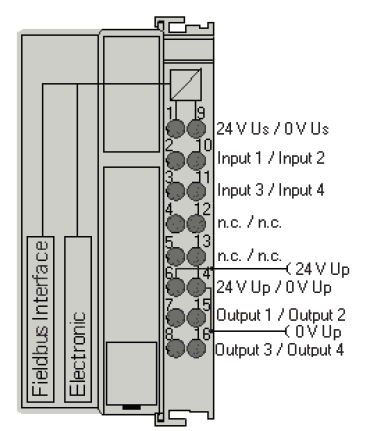
\includegraphics[scale=0.6]{Immagini/Sperimentale/Beckoffschema.PNG}
		\caption{Schema modulo bechoff}
		\label{fig:ModuloBechoff}
	\end{center}
\end{figure}
\subsubsection{Configurazione della rete}
La configurazione della rete prevede alla base il PC Target, in questo vi è una chiavetta USB che fa \textit{runnare} sul pc un sistema operativo simulink real time. Il target è il master della rete, ha due uscite ethernet, la prima è collegata direttamente al modulo bechkoff, il quale prende l'identità di primo slave, e come visto precedentemente, al bechkoff sono attaccati e i due azionamenti che si comportano come slave aggiuntivi.
\begin{figure}[ht]
\begin{center}
    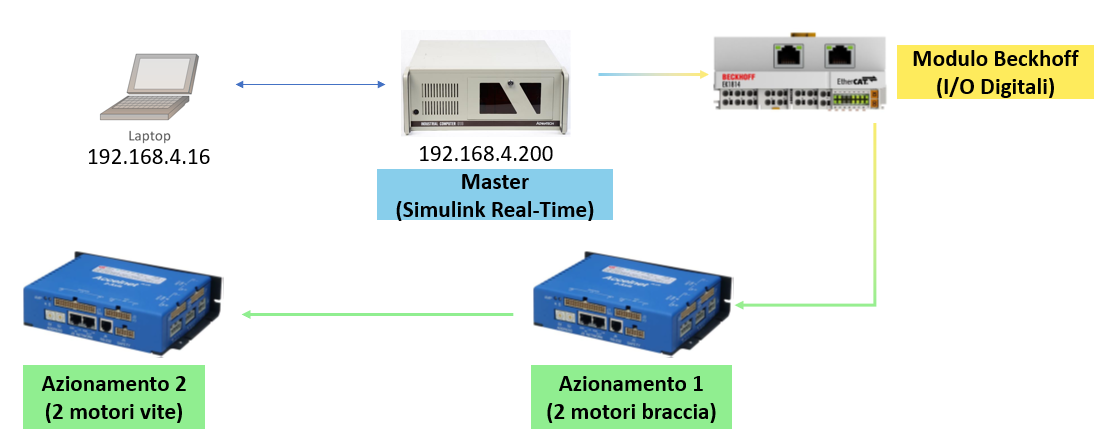
\includegraphics[scale=0.5]{Immagini/Sperimentale/Topology.PNG}
    \caption{Topologia della rete}
    \label{fig:NetTopology1}
\end{center}
\end{figure}
\\Alla seconda porta ethernet, vi è collegato il PC dell'utente, il quale provvede a generare, compilare, e caricare i programmi sul PC target. Da User-PC è anche possibile vedere i grafici e fare delle analisi sulle movimentazioni e le traiettorie eseguite dal manipolatore. La connessione avviene tramite una rete ethernet, l'indirizzo del target è 192.168.4.200, invece per User-PC:
\begin{figure}[ht]
\begin{center}
    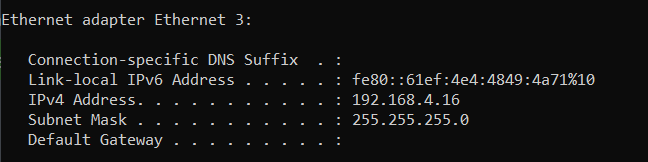
\includegraphics[scale=0.7]{Immagini/Sperimentale/ConfEthernet.png}
    \caption{Configurazione rete ethernet user PC}
    \label{fig:ConfEthernet}
\end{center}
\end{figure}
\\Va precisato che il pc dell'utente non fa parte della rete ethercat, ma la rete inizia soltanto dal pc target in poi, infatti, ad esclusione delle operazioni viste precedentemente il manipolatore non ha bisogno del pc utente per funzionare.
\begin{figure}[ht]
	\begin{center}
		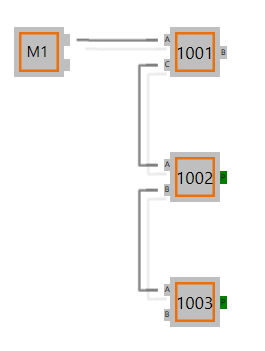
\includegraphics[scale=0.7]{Immagini/Sperimentale/NetTopology.png}
		\caption{Topologia rete mediante Ec-engineer}
		\label{fig:NetTopology2}
	\end{center}
\end{figure}
\\Una volta configurata la rete, il passo successivo è quello della configurazione dei messaggi, come anticipato nel capitolo precedente il metodo di comunicazione sono le PDO. Le PDO possono essere in input o in output, la differenza sta nel fatto che le prime sono trasmesse al master dagli azionamenti, di conseguenza il master le riceve, quelle in output invece sono PDO che il master trasmette e che gli azionamenti ricevono. 
\\Nelle immagini seguenti vengono mostrate le PDO di input, in particolare:
\begin{itemize}
 	\item PDO1 e PDO2 contengono i parametri di posizione, velocità coppia effettiva e modalità operativa che vengono trasmesse dagli azionamenti
 	\item PDO3, contiene input generici che sono indipendenti dalla modalità operativa del motore, in particolare è presente il \textit{general purpose inputs} che è il registro che permette la visione dei finecorsa
 	\item PDO4 contiene \textit{status word} e \textit{control word}, sono registri importanti che servono per verificare la modalità operativa e lo stato dell'azionamento, quindi sono utili per capire se l'azionamento è in fase pre-operativa, operativa o in errore
\end{itemize}
\begin{figure}[!ht]
\begin{subfigure}{.5\textwidth}
  \centering
  % include first image
  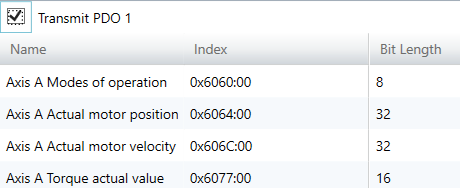
\includegraphics[width=.7\linewidth]{Immagini/Sperimentale/pdo1in.png}  
  \caption{PDO Input 1}
  \label{fig:sub-firstpdo}
\end{subfigure}
\begin{subfigure}{.5\textwidth}
  \centering
  % include second image
  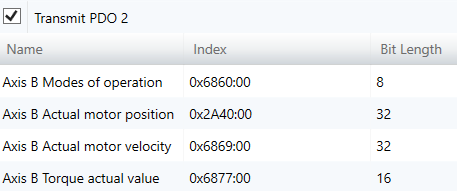
\includegraphics[width=.7\linewidth]{Immagini/Sperimentale/pdo2in.png}  
  \caption{PDO Input 2}
  \label{fig:sub-secondpdo}
\end{subfigure}
\begin{subfigure}{.5\textwidth}
  \centering
  % include third image
  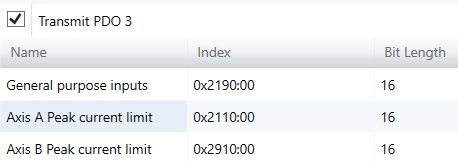
\includegraphics[width=.7\linewidth]{Immagini/Sperimentale/pdo3in.png}  
  \caption{PDO Input 3}
  \label{fig:sub-thirdpdo}
\end{subfigure}
\begin{subfigure}{.5\textwidth}
  \centering
  % include fourth image
  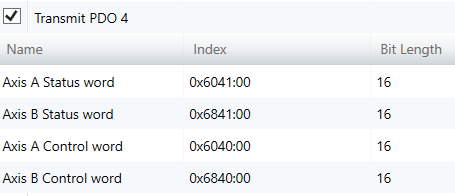
\includegraphics[width=.7\linewidth]{Immagini/Sperimentale/pdo4in.png}  
  \caption{PDO Input 4}
  \label{fig:sub-fourthpdo}
\end{subfigure}
\caption{PDO in input}
\label{fig:PDOIn}
\end{figure}
Per quanto riguarda le PDO in output che riceve l'azionamento sono solo due, ed i parametri ricevuti sono:
\begin{figure}[ht]
	\begin{center}
		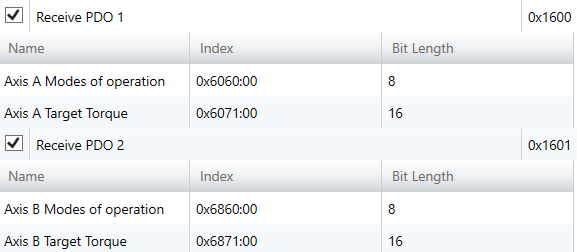
\includegraphics[scale=0.6]{Immagini/Sperimentale/pdo12out.png}
		\caption{PDO Output 1 e 2}
		\label{fig:PDOOut}
	\end{center}
\end{figure}
\begin{itemize}
	\item \textit{Modes of operation}, è un registro che specifica la modalità con la quale verrà controllato l'azionamento, per esempio coppia, posizione, velocità o ciclica
	\item \textit{Target torque}, specifica il valore di coppia che l'azionamento dovrà fornire al motore
\end{itemize}
\subsection{Implementazione nel sistema reale}
Una volta ottenuto il file ENI contenente la topologia della rete è stato utilizzato simulink real-time per implementare la logica di controllo del manipolatore
\begin{figure}[ht]
	\begin{center}
		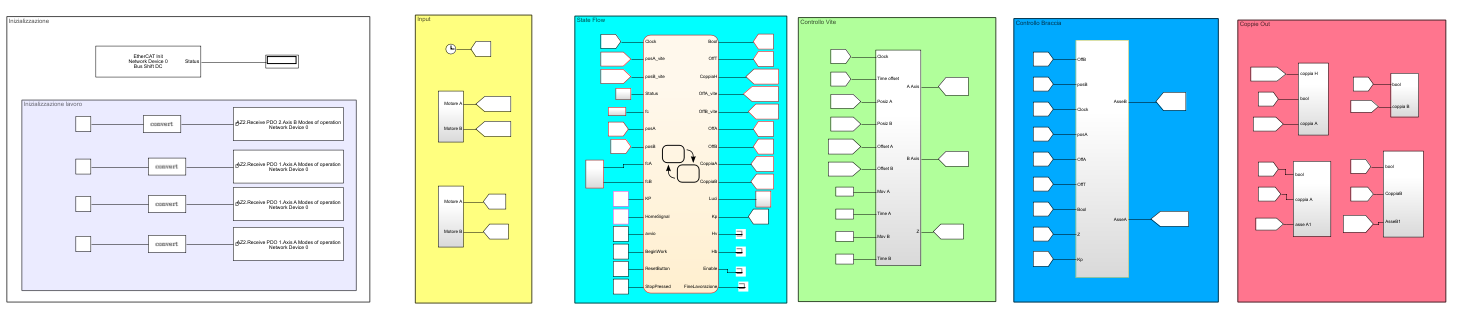
\includegraphics[scale=0.5]{Immagini/Sperimentale/generalSchema}
		\caption{Schema generale simulink}
		\label{fig:SimulinkSchema}
	\end{center}
\end{figure}
\\Il programma è stato diviso in sei stati diversi, si presentano e analizzano ora i vari stati.
\subsubsection*{Inizializzazione}
\addcontentsline{toc}{subsubsection}{Inizializzazione}
La prima fase è quella di inizializzazione, in questa fase viene inserito il file ENI e viene specificata la modalità operativa degli azionamenti.
\begin{figure}[ht]
	\begin{center}
		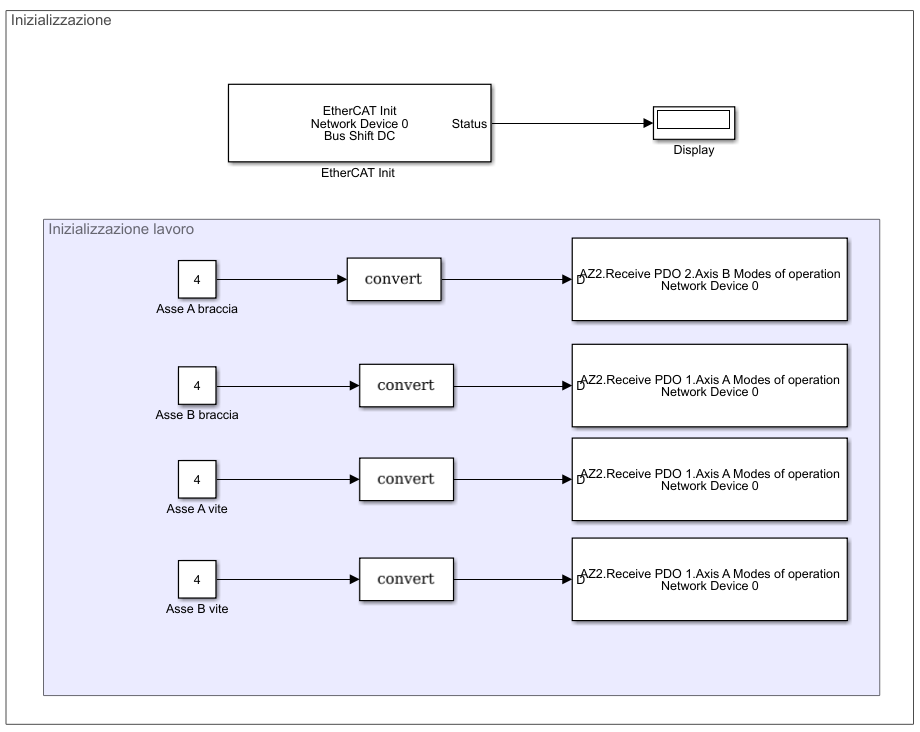
\includegraphics[scale=0.63]{Immagini/Sperimentale/Inizializzazione}
		\caption{Fase 1: Inizializzazione}
		\label{fig:Init}
	\end{center}
\end{figure}
Oltre al file ENI viene anche specificata la porta di comunicazione ed il bus che verranno utilizzati per lo scambio di dati. Ogni azionamento ha poi una determinata modalità operativa, come visto nelle sezioni precedenti il controllo è effettuato in coppia (mod. 4). 
\begin{table}[h!]
	\centering
	\begin{tabular}{|c |c|} 
		\hline
		Modalità & Descrizione  \\ 
		\hline
		1 & modalità profilo in posizione  \\ 
		3 & modalità profilo in velocità  \\
		4 & modalità profilo in coppia   \\
		6 & modalità homing \\
		7 & modalità posizione interpolata\\
		\hline
	\end{tabular}
	\caption{Tipologie controllo azionamenti}
	\label{table:5}
\end{table}
\subsubsection*{Input}
\addcontentsline{toc}{subsubsection}{Input}
La seconda fase è quella di input, in questa fase vengono presi tutti i valori di posizione dei motori sia della vite che delle braccia. I valori vengono presi mediante lo scambio di PDO ed hanno bisogno di essere convertiti, proprio per questo la struttura di ricezione di un messaggio è la seguente: 
\begin{figure}[ht]
	\begin{center}
		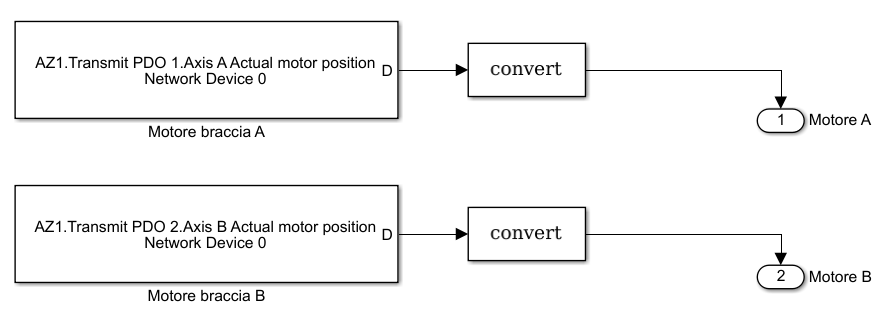
\includegraphics[scale=0.6]{Immagini/Sperimentale/convertS}
		\caption{Conversione e lettura motori}
		\label{fig:MotorConversion}
	\end{center}
\end{figure}
\\Nella figura successiva è possibile vedere la struttura del blocco di ricezione degli input, tutti i valori dopo una conversione entrano in blocchi \textit{goto} e vengono ripescati negli stati successivi da blocchi \textit{from}.
\begin{figure}[ht]
	\begin{center}
		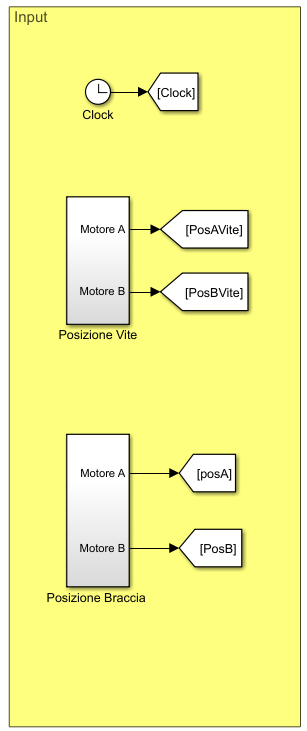
\includegraphics[scale=0.7]{Immagini/Sperimentale/Input}
		\caption{Fase 2: Input}
		\label{fig:Input}
	\end{center}
\end{figure}
\subsubsection*{Stateflow}
\addcontentsline{toc}{subsubsection}{Stateflow}
Il blocco stateflow è un blocco è posta la logica fondamentale dell'applicazione, in ingresso si hanno dati che servono per il controllo delle traiettorie e degli stati del manipolatore, in particolare il clock, lo stato dei finecorsa, le posizioni dei motori e delle variabili di input che serviranno per gestire interamente l'interfaccia grafica. In uscita si hanno gli offset, utili per avere un riferimento spaziale di posizione e temporale, in quanto aiutano a capire di quanto e quanto tempo il manipolatore si è mosso, le coppie di \textit{homing} dei motori, un blocco per la gestione delle luci e variabili di output che serviranno per l'accensione e lo spegnimento dei led nell'interfaccia grafica.
\begin{figure}[ht]
	\begin{center}
		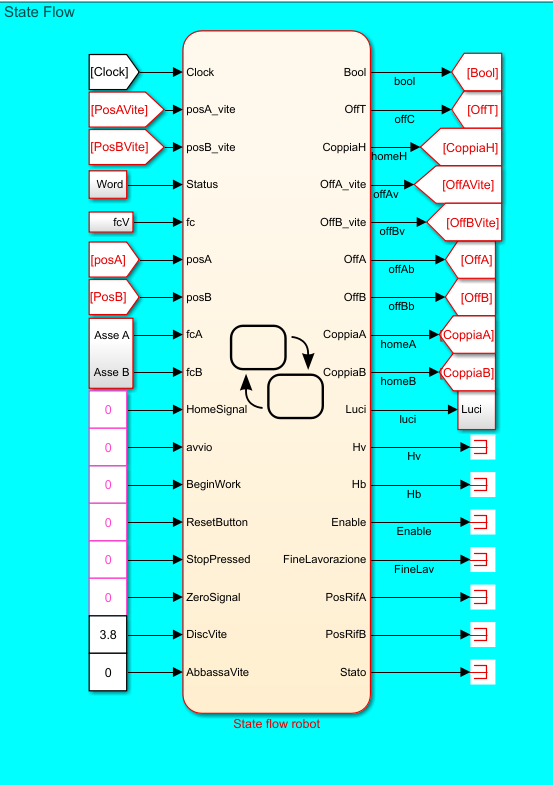
\includegraphics[scale=0.84]{Immagini/Sperimentale/sf0new}
		\caption{Fase 3: Stateflow}
		\label{fig:Stateflow1}
	\end{center}
\end{figure}
\subsubsection*{Controllo vite}
\addcontentsline{toc}{subsubsection}{Controllo vite}
Il blocco Controllo Vite, contiene lo schema del controllore implementato per controllare la vite, in ingresso si hanno variabili come il clock, le posizioni dei motori con relativi offset e la movimentazione da far eseguire ad entrambi i motori con il tempo di esecuzione.
\begin{figure}[ht]
	\begin{center}
		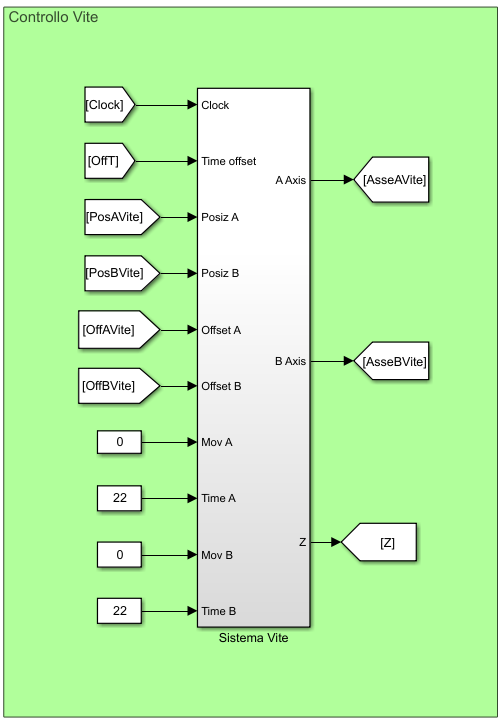
\includegraphics[scale=0.7]{Immagini/Sperimentale/ControlloViteSchema}
		\caption{Fase 4: Schema di controllo della vite}
		\label{fig:ControlloVite}
	\end{center}
\end{figure}
Grazie a tutti questi parametri è possibile definire le leggi di moto che permettono di eseguire il movimento nell'asse Z. Importante è sapere che il movimento eseguito dalla vite a ricircolo di sfere è dipendente anche da quello della guida lineare, infatti la rotazione provoca anche un abbassamento della vite, per risolvere questo problema il motore della guida dovrà essere sempre pronto a rispondere e correggere questa situazione; in caso che i due motori vadano alla stessa velocità si avrà una rotazione senza traslazione.
\subsubsection*{Controllo braccia}
\addcontentsline{toc}{subsubsection}{Controllo braccia}
Il blocco Controllo Braccia è quello responsabile della movimentazione dei link motorizzati, come per il blocco della vite prende in ingresso le posizioni, il \textit{clock} con i relativi offset ed internamente vengono svolte le operazioni di selezione della traiettoria, generazione della legge di moto con conseguente creazione degli angoli di riferimento (grazie alle relazioni di cinematica e dinamica) ed implementazione dello schema di controllo. In uscita si avranno le coppie da assegnare ai due motori delle braccia.
\begin{figure}[ht]
	\begin{center}
		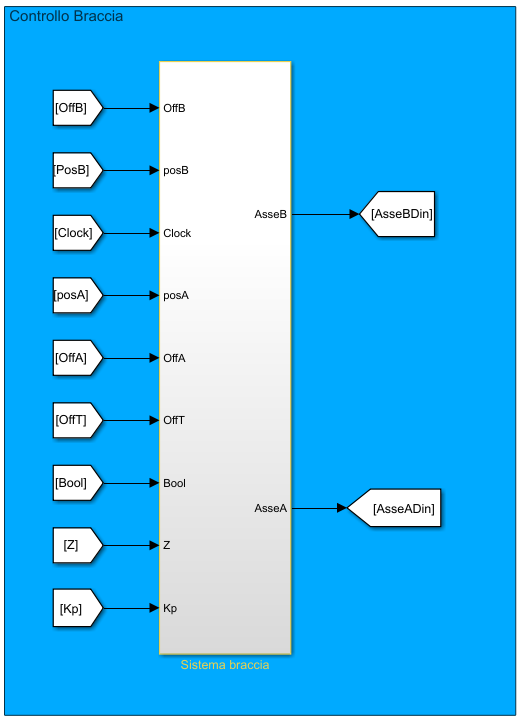
\includegraphics[scale=0.75]{Immagini/Sperimentale/ControlloBraccia}
		\caption{Fase 5: Schema di controllo delle braccia}
		\label{fig:controlloBraccia}
	\end{center}
\end{figure}
La scelta di dividere il controllo delle braccia e quello della vite in due blocchi diversi è stata fatta in quanto i due sono indipendenti l'uno dall'altro. Inizialmente il focus è stato posto sul controllo della vite, per poi passare a quello delle braccia ed infine dopo vari test i due controlli sono stati implementati contemporaneamente.
\subsubsection*{Coppie uscita}
\addcontentsline{toc}{subsubsection}{Coppie uscita}
Dopo aver ottenuto le coppie di homing dallo stateflow e le coppie dei motori dagli schemi di controllo è venuto il momento di inviare le coppie agli azionamenti e di conseguenza ai motori; per far questo viene utilizzato un blocco per ogni motore, oltre alle coppie in entrata avremo anche una variabile di controllo. 
\begin{figure}[ht]
	\begin{center}
		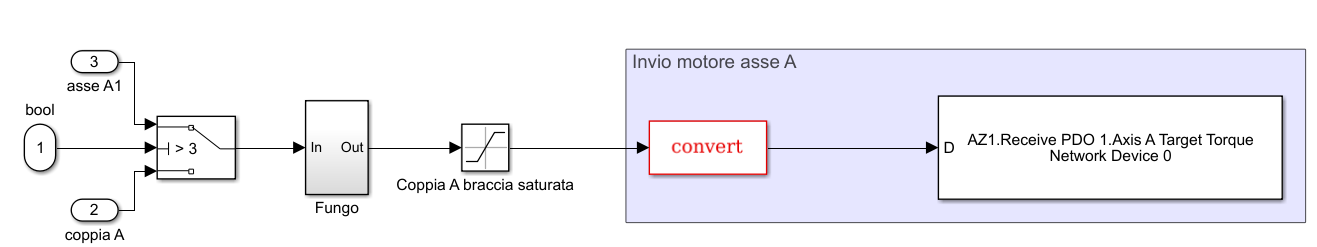
\includegraphics[scale=0.55]{Immagini/Sperimentale/Saturatore}
		\caption{Schema espanso invio coppia}
			\label{fig:CoppieoutExpanded}
	\end{center}
\end{figure}
Nella figura precedente è possibile vedere lo schema espanso come spiegato, lo \textit{switch} permette la scelta in base alla variabile bool, fintanto che è minore o uguale a 3 verrà erogata solo la coppia di Homing, quando arriva a 4 invece vuol dire che si è nella fase di controllo, di conseguenza verrà erogata la coppia di controllo. Successivo allo switch c'è un blocco che serve per la gestione delle emergenze, infatti, una volta premuto il fungo verrà assegnata una coppia costante uguale a 0 che fermerà la lavorazione ed anche dopo che verrà sbloccato il fungo la coppia per sicurezza rimarrà a zero, l'unico modo per resettare questa condizione è il riavvio del programma.
\begin{figure}[ht]
	\begin{center}
		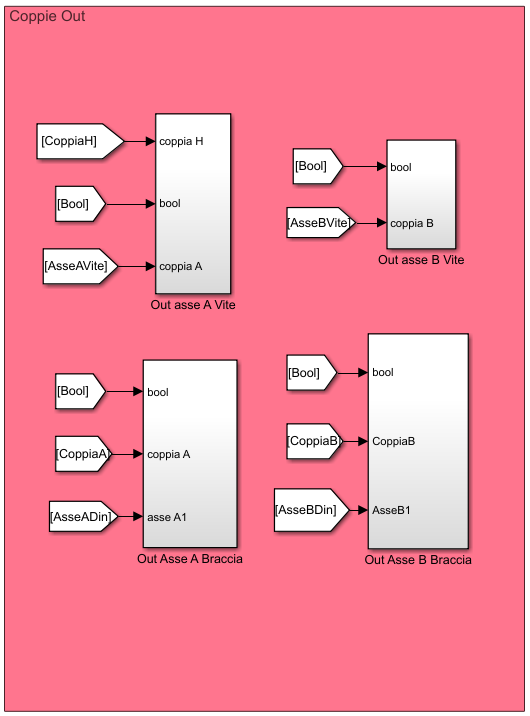
\includegraphics[scale=0.6]{Immagini/Sperimentale/CoppieOut}
		\caption{Fase 6: Copie in uscita
			\label{fig:Coppieout}}
	\end{center}
\end{figure}
\\Successivo al blocco fungo vi è la presenza di un saturatore, questo serve per evitare di danneggiare il manipolatore in caso che le coppie computate siano molto alte, è stato trovato sperimentalmente un limite che coincide con la coppia nominale che non può essere superato, per concludere l'ultima parte è quella che si occupa di inviare mediante PDO il valore di coppia convertito all'azionamento.La trattazione andrà a concentrarsi sulle parti principali di questo programma, in particolare andremo a trattare lo stateflow il metodo di funzionamento ed i vari stati, passeremo poi all'interfaccia grafica che permette di comandare il manipolatore, e per concludere andremo a vedere i controllori implementati per la vite e per le braccia, andando a vedere la struttura, lo schema e i risultati ottenuti per ogni approccio.
\subsection{Stateflow}
\textit{Stateflow} si occupa di fornire diagrammi di transizione, di stato e di flusso utilizzando un linguaggio grafico. Nel caso del manipolatore è stato utilizzato per la progettazione dei diagrammi di transizione in base agli stati del robot. In questa sezione andremo a vedere le fasi gli stadi di evoluzione che sono stati costruiti, per comodità si fa riferimento allo schema seguente:
\begin{figure}[ht]
	\begin{center}
		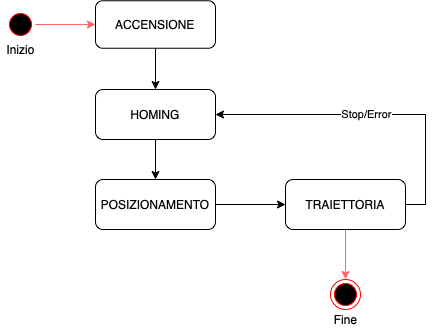
\includegraphics[scale=0.6]{Immagini/Sperimentale/statemachine}
		\caption{Macchina a stati stateflow
			\label{fig:macchinaStati}}
	\end{center}
\end{figure}
\subsubsection{Fase di Homing}
Appena il robot viene acceso non vi è alcuna conoscenza relativa alla sua posizione, di conseguenza è necessario avere uno stadio che lo porti in una posizione di riferimento nella quale è nota la collocazione effettiva. Il primo stadio è quindi quello di \textit{homing}, consiste nel portare i motori a toccare i finecorsa indicando quello come punto di partenza. I motori utilizzati per questa fase sono stati quelli delle braccia e quello di traslazione della vite.
\par L'approccio iniziale è stato quello di fornire una coppia costante che in automatico si occupava di andare a toccare i finercorsa, dopo che erano stati toccati si passava nello stato successivo. Però, per motivi di sicurezza e, considerando che lasciando fermo il manipolatore per diverso tempo la stessa coppia costante potrebbe non essere in grado di farlo muovere si è deciso di chiudere l'anello in posizione, in particolare per eseguire la fase di \textit{homing} è stata data in ingresso una rampa con pendenza negativa\footnote{i finecorsa utilizzati per questa fase vengono rilevati quando i link sono totalmente a destra, quindi la direzione negativa per i motori delle braccia.}.
Per controllare la rampa è stato fatto un controllo proporzionale e integrale sull'errore tra la posizione attuale ed il riferimento, la legge di controllo implementata è del tipo:
\begin{equation*}
	PI = \frac{K_p s + K_i}{s}
\end{equation*}
Nella figura \ref{fig:Zero} è possibile vedere lo schema implementato per questa prima fase:
\begin{figure}[ht]
\begin{center}
    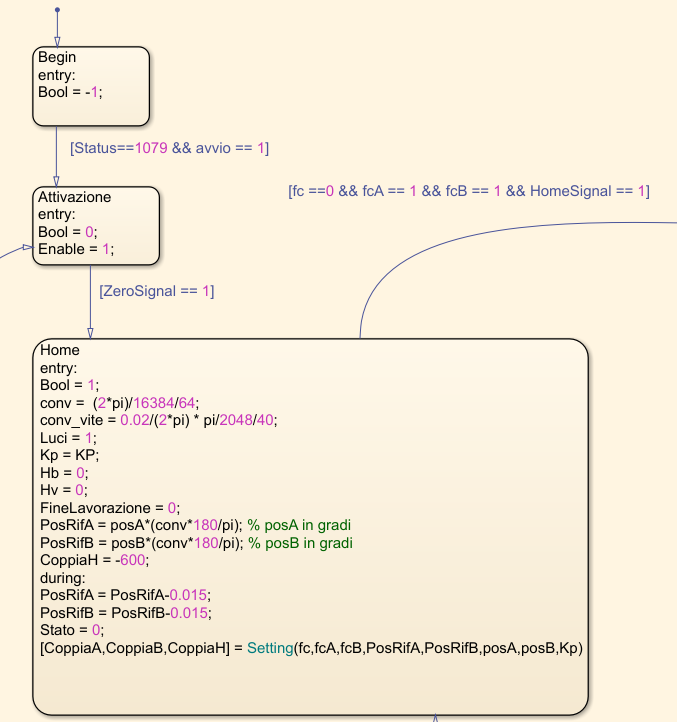
\includegraphics[scale=0.8]{Immagini/Sperimentale/state1new.png}
    \caption{Fase di Homing}
    \label{fig:Zero}
\end{center}
\end{figure}
\\Il primo stato è quello di \textbf{Begin}, appena il programma si avvia si entra in automatico nello stato, per passare allo stato successivo, ovvero \textbf{Attivazione} vanno soddisfatte due condizioni, la prima si verifica quando la \textit{Status Word} è uguale a 1079, ovvero quando gli azionamenti sono usciti dalla fase \textit{pre-operational} e sono quindi pronti all'uso, la seconda invece quando il segnale avvio è vero. Nello stato attivazione i motori sono ancora fermi però viene abilitato il loro utilizzo, passare quindi in questo stato è obbligatorio. Si passa nello stato successivo quando il segnale \textit{ZeroSignal} è vero, questo viene gestito mediante un bottone da interfaccia grafica, appena premuto si entra automaticamente nello stato \textbf{Home}. 
\par In questo stato vengono definite le variabili per la conversione dei valori presi dai motori\footnote{I valori sono espressi tutti in \textit{counts},  è stata necessaria una fase di analisi dei motori per capire come convertirli, effettuando quindi un passaggio da \textit{counts} a radianti e da radianti a gradi.}, viene poi salvata la posizione di riferimento degli assi A e B dei motori delle braccia. La fase successiva è quella del \textit{during}\footnote{Finché si rimane in quello stato, le operazioni vengono eseguite ad ogni ciclo (1ms).}, in questa si ha che la rampa decresce di 0.015 gradi al millisecondo, quindi 15 gradi al secondo e successivamente una funzione simulink che si occupa del controllo PI. Una volta raggiunta la posizione del finecorsa le coppie vengono settate a 0, impedendo quindi un'ulteriore movimentazione,oltre al movimento delle braccia c'è anche quello della vite, che raggiunge la posizione di Homing salendo con una coppia negativa. Per passare alla fase successiva è necessario che tutti gli elementi siano arrivati a finecorsa.
\subsubsection{Fase di posizionamento}
La fase successiva è quella di posizionamento, per non lasciare il robot nella configurazione di homing si è scelto di spostarlo in una configurazione standard lontana dai punti di singolarità che sarà comoda per le movimentazioni successive. La configurazione scelta prevede che i giunti siano messi a $100^\circ$ e $80^\circ$, anche in questo caso, come prima il primo approccio è stato quello di utilizzare una coppia costante per il movimento; la fase di homing lasciava i link a $60^\circ$ e $-30^\circ$, vi era quindi la necessità di fare $+40^\circ$ per il braccio sinistro e $+110^\circ$ per quello destro, la coppia costante veniva erogata finché la condizione non era vera, dopodiché vi era la sicurezza che il posizionamento fosse stato effettuato in maniera corretta. 
\par L'approccio di posizionamento finale però non è stato quello della coppia costante, anche in questo caso per motivi di sicurezza ma, sapendo le posizioni finali che si vogliono raggiungere, si è optato per definire una legge di moto che si occupa di portare il manipolatore nella condizione desiderata.
\begin{figure}[ht]
\begin{center}
    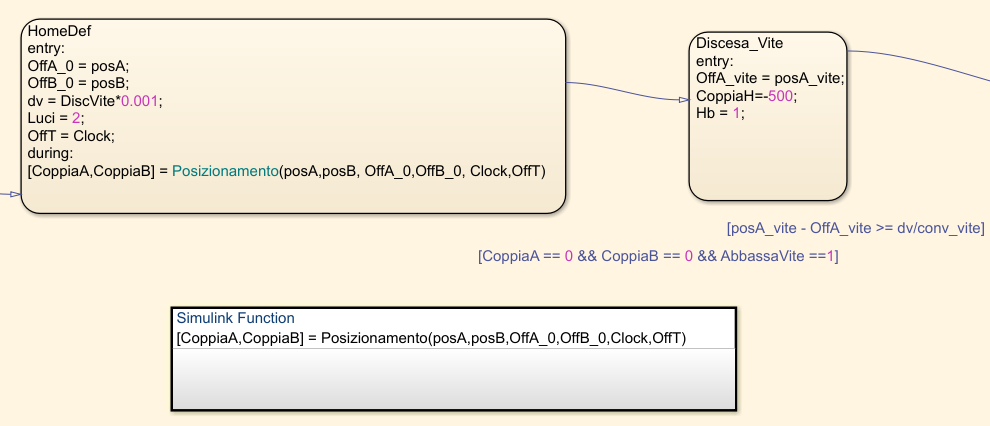
\includegraphics[scale=0.65]{Immagini/Sperimentale/state2New.png}
    \caption{Fase di posizionamento}
    \label{fig:Pos}
\end{center}
\end{figure}
\\A partire dallo schema precedente, per passare allo stato \textbf{HomeDef} bisogna aver raggiunto tutti i finecorsa; non appena si entra nello stato vengono salvati gli offset della posizione delle braccia, del tempo e la posizione desiderata di discesa della vite. Ad ogni ciclo, quindi ogni millisecondo viene eseguita la funzione \textbf{Posizionamento($\dots$)} la quale, mediante una legge di moto, consente di eseguire in maniera corretta il posizionamento.
Analizzando nello specifico il blocco simulink del posizionamento, vengono costruite due leggi polinomiali, una per ogni motore che producono un \textit{setpoint} in posizione in gradi, che verrà confrontato con la posizione attuale. Per ottenere la coppia, e garantire errore a transitorio esaurito viene introdotto un sistema di controllo proporzionale integrativo, con legge di controllo: 
% check formula
\begin{equation*}
\tau = K \tilde{\theta} =  K_p\tilde{\theta} + K_i\tilde{\theta}
\end{equation*}
Le coppie di controllo uscenti andranno al manipolatore e si occuperanno della movimentazione. È possibile vedere lo schema della legge di moto implementato in figura \ref{fig:ImpPos}.
\begin{figure}[ht]
	\begin{center}
		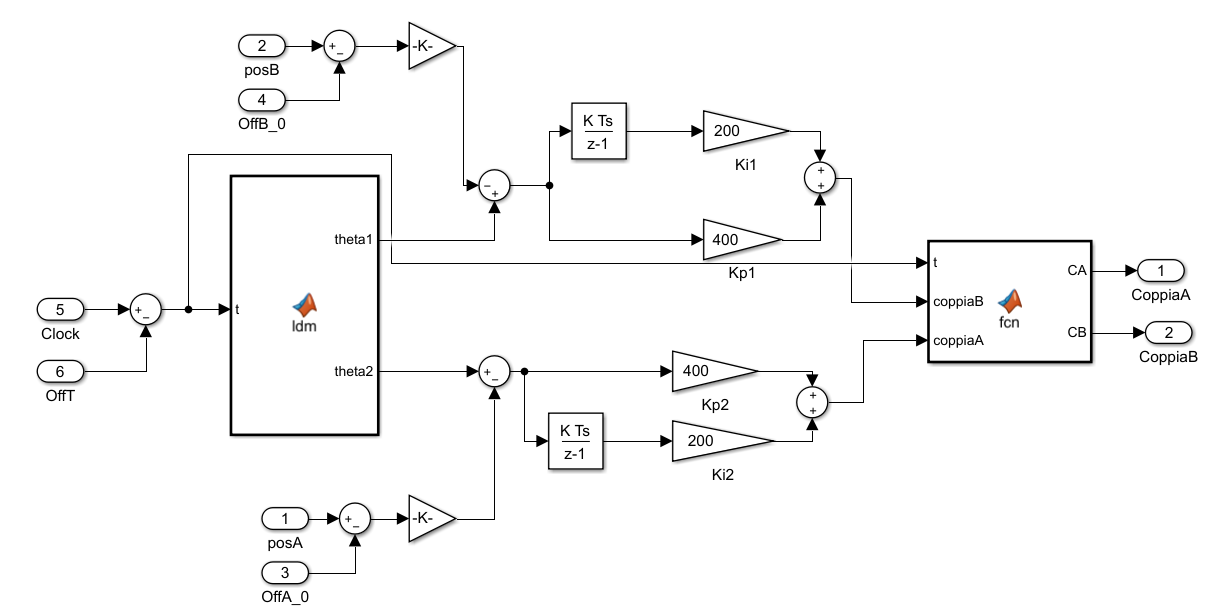
\includegraphics[scale=0.6]{Immagini/Sperimentale/LdmPosizionamento}
		\caption{Implementazione funzione di posizionamento}
		\label{fig:ImpPos}
	\end{center}
\end{figure}
Per quanto riguarda la vite sono state implementate due possibili scelte: la prima è l'opzione di farla abbassare la seconda invece è quella di lasciarla in posizione di finecorsa, si è scelto di proseguire in questo modo in quanto per vite come visto precedentemente nel capitolo \ref{DescrizioneEF},  è possibile collegare utensili e quindi l'abbassamento di una determinata quantità la predispone al disegno per traiettorie bidimensionali. 
Una volta eseguito il posizionamento, lo stato successivo riguarda la discesa della vite, per entrarci le coppie delle braccia dovranno essere pari a zero e sull'interfaccia grafica dovrà essere premuto il bottone relativo all'abbassamento della vite\footnote{Sia che si voglia abbassare di una quantità che si voglia lasciare nella posizione alta il bottone va premuto.}. Per particolare per la discesa verrà utilizzata la variabile \textbf{dv} salvata precedentemente che indica di quanti centimetri la vite deve scendere; per farla scendere viene fornita una coppia al motore di traslazione finché non arriva alla posizione desiderata.
\subsubsection{Fase di controllo}
L'ultima fase è quella di controllo ed esecuzione della traiettoria, in questa fase si procede settando l'offset dei motori della vite, del tempo e dei motori delle braccia; resettare l'offset della vite è necessario in quanto il posizionamento (nel caso di discesa) è appena terminato; l'offset del tempo permette di far partire virtualmente il tempo da zero negli schemi di controllo dopo essere arrivati nella configurazione di \textit{Posizionamento}. I figura \ref{fig:Traiettoria} lo schema implementato di quest'ultima fase.
\begin{figure}[ht]
\begin{center}
    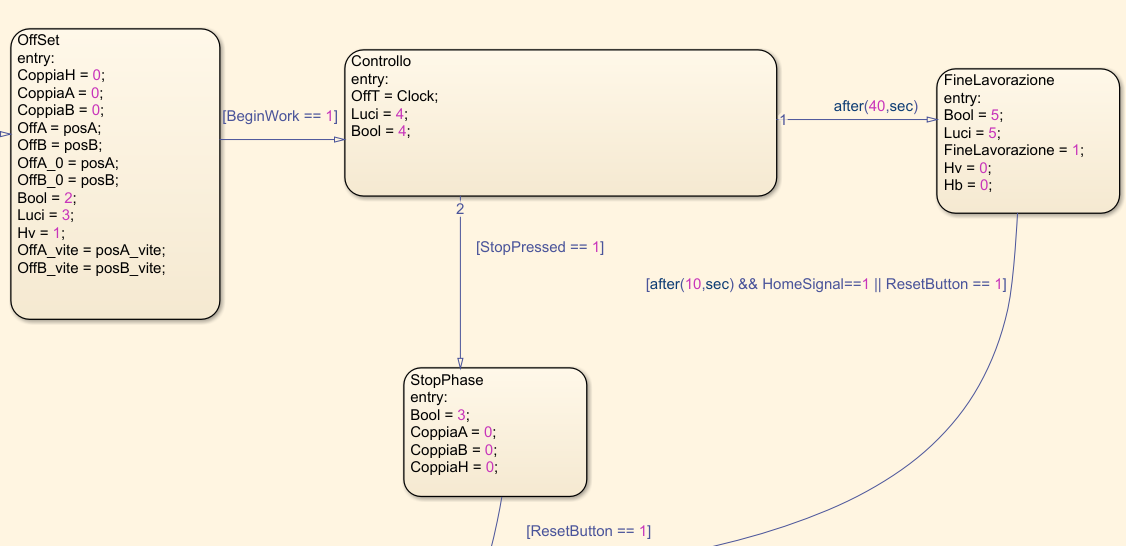
\includegraphics[scale=0.6]{Immagini/Sperimentale/state3New.png}
    \caption{Fase di controllo}
    \label{fig:Traiettoria}
\end{center}
\end{figure}
\par Come anticipato precedentemente nello stato \textbf{OffSet} avviene il settaggio degli \textit{offset} e tutte le coppie vengono messe a zero per evitare eventuali movimentazioni indesiderate. Per passare alla fase successiva vi è la necessità che venga premuto il bottone \textbf{Work} sull'interfaccia grafica, questo garantisce il passaggio allo stato \textit{Controllo}, può darsi che il bottone non venga premuto subito, di conseguenza il clock potrebbe aumentare, per questo l'offset viene settato nella fase di \textbf{Controllo}. Per quanto riguarda la scelta della traiettoria tramite interfaccia grafica vi è la possibilità di scegliere quella desiderata. A livello di implementazione le traiettorie non sono altro che leggi di moto costruite in due o tre dimensioni. Dopo che il manipolatore inizia ad eseguire la traiettoria possono esserci due evoluzioni:
\begin{itemize}
	\item la traiettoria viene eseguita correttamente
	\item la traiettoria da problemi
\end{itemize}
Nel primo caso si ha un tempo 40 secondi per eseguire la traiettoria (il tempo può essere personalizzato in base alla tipologia di traiettorie), alla fine di questo tempo si passa nello stato \textbf{FineLavorazione} dove il manipolatore è fermo ed ha concluso la sua traiettoria, da questo, grazie al bottone reset è possibile ritornare alla fase di \textbf{homing}, oppure in automatico dopo un determinato periodo di tempo se il tasto di \textit{posizionamento} è stato lasciato attivo il manipolatore torna nella configurazione predefinita. Nel secondo caso si nota che la traiettoria sta dando problemi, ad esempio vibrazioni o si nota che il manipolatore rischia di entrare in singolarità, per risolvere questi problemi vi è un bottone denominato \textbf{STOP} che permette l'arresto immediato del manipolatore, azzerando tutte le coppie. A differenza della pressione del fungo, che dopo lo sbloccaggio richiede il riavvio del dispositivo, nel caso in cui si entri nella fase di stop mediante il bottone di reset è possibile far tornare il manipolatore nella fase di attivazione, da questa poi sarà possibile far partire di nuovo la fase di homing e successivamente quella di posizionamento.
\subsubsection*{Gestione variabile di stato e luci}
\addcontentsline{toc}{subsubsection}{Gestione variabile di stato e luci}
Durante tutte le fasi è possibile vedere nello stateflow che due variabili si evolvono costantemente: bool e luci.
\\La prima serve per indicare lo stato di lavoro nel quale si trova il manipolatore, in particolare l'evoluzione segue la tabella degli stati \ref{table:3}.
\begin{table}[h!]
\centering
\begin{tabular}{|c |c |} 
 \hline
 Valore & Stato \\ [0.5ex] 
 \hline\hline
  -1  & Pre-operativo \\ 
  0  & Attivo \\
  1 & Homing \\
  2 & Manipolatore posizionato\\
  3 & Traiettoria\\
  4 & Fine lavorazione \\
 \hline
\end{tabular}
\caption{Valori variabile \textit{bool}}
\label{table:3}
\end{table}
\\Il valore di luci, serve esattamente a pilotare le luci presenti nel manipolatore\footnote{Inizialmente le luci erano solo fisiche, montate nella parte posteriore del manipolatore, per comodità visiva sono state anche implementate nell'interfaccia grafica.}  secondo la tabella \ref{table:luci}, in modo tale da avere un feedback visuale che indica fase in cui è il manipolatore.
\begin{table}[h!]
\centering
\begin{tabular}{|c |c|c|} 
 \hline
 Valore & Colore & Bool \\ [0.5ex] 
 \hline\hline
  1  & Bianco & 1 \\ 
  2 &  Bianco Rosso & 1\\
  3 &  Rosso & 2 \\
  4 & Bianco Verde & 3\\
  5 & Verde & 4\\
 \hline
\end{tabular}
\caption{Valori luci}
\label{table:luci}
\end{table}
\subsubsection{Interfaccia grafica}
Per gestire al meglio le varie impostazioni, e per essere sicuri del passaggio tra i vari stati è stata creata un'interfaccia grafica \textit{user-friendly} mediante \textit{instrument panel} fornito da \textit{Simulink real-time explorer}, è possibile vederla in figura \ref{fig:gui}.
\begin{figure}[ht]
	\begin{center}
		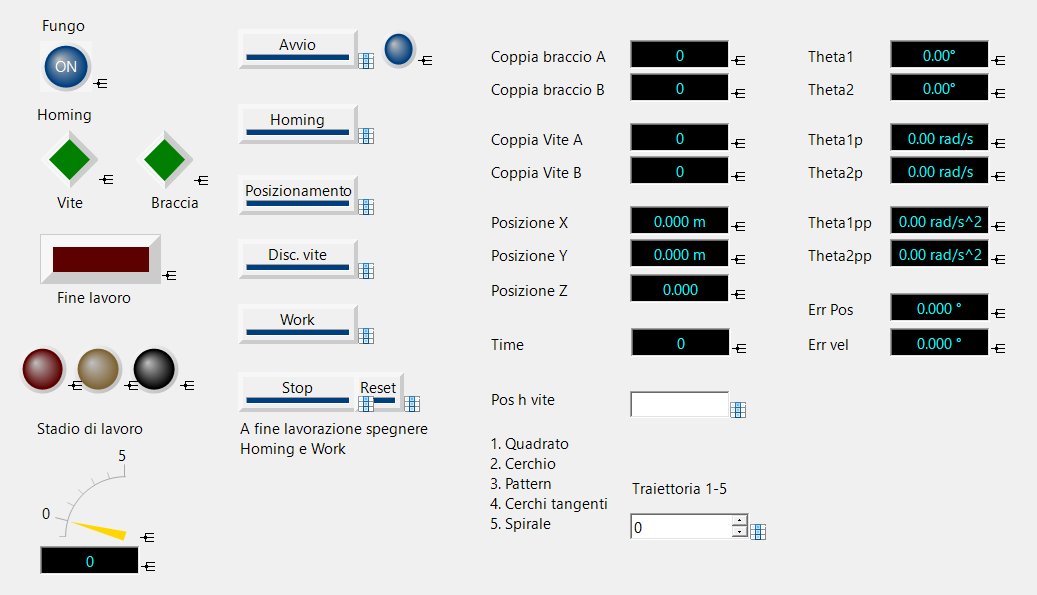
\includegraphics[scale=0.6]{Immagini/Sperimentale/GUI3}
		\caption{Interfaccia grafica}
		\label{fig:gui}
	\end{center}
\end{figure}
\\A sinistra, dall'alto in basso sono presenti dei LED che hanno la funzionalità di:
\begin{itemize}
	\item Fungo: rimane acceso fintantoché il fungo non è premuto
	\item Homing: si accendono quando i motori hanno raggiunto il finecorsa
	\item Fine lavoro: appena la traiettoria assegnata finisce questo si accende
	\item Luci: sono i led visti nella tabella \ref{table:luci}, che vanno ad indicare in che fase di lavoro è il manipolatore, per comodità visiva il led bianco nell'interfaccia è stato sostituito da uno ocra
\end{itemize} 
Sotto questi led vi è un indicatore che va a specificare le fasi di lavoro come viste nella tabella \ref{table:3}. Al centro sono presenti i bottoni che permettono di passare tra le varie fasi dello stateflow e di fare tutte le operazioni quindi avvio, homing, posizionamento, lavoro stop e reset. In particolare i bottoni funzionano tramite il collegamento a determinate variabili; quelle di riferimento sono le ultime costanti collegate in input allo stateflow visto in figura \ref{fig:Stateflow1}. A destra c'è invece una parte di visualizzazione dove è possibile vedere tutti i parametri di interesse del manipolatore, in particolare le coppie fornite e le posizioni sia nel piano $[x,y,z]$ che quelle ai link motorizzati quindi $\theta_1,\theta_2$. Infine, è presente il selettore di traiettoria, il quale permette la scelta fra le sei opzioni possibili (di default viene eseguito il cerchio).
\begin{enumerate}
	\item Quadrato
	\item Cerchio
	\item Pattern
	\item Cerchi tangenti
	\item Spirale
	\item Solo asse Z
\end{enumerate}
Adesso che è stata introdotta la logica di funzionamento a stati, è possibile proseguire la trattazione andando a vedere le tipologie di controllo che sono state implementate, in particolare inizieremo col guardare il controllo applicato alla vite e successivamente quello per le braccia.
\subsection{Controllo vite}%CHECK
Lo scopo di questa sottosezione è quello di introdurre le due tipologie di controllo per la vite, da un punto di vista teorico e andare ad analizzare il comportamento pratico. Il sistema, essendo formato da due parti, e potendo fare solo due movimenti è ad un solo grado di libertà non risulta essere quindi molto complesso. Gli approcci di controllo utilizzati sono di tipo centralizzato, l'analisi di questi controllori verrà fatta mediante funzioni di trasferimento, per proseguire con la discussione viene introdotta la legge di controllo di un controllore PID generico:
\begin{equation}
\tau_v (t) = K_p \bigg(q_v(t) + \frac{1}{T_I} \int_0^t q_v(\tau) d\tau + T_D \frac{d q_v(t)}{dt}\bigg)
\label{eq:PID}
\end{equation}
\subsubsection{Controllo proporzionale}
Il primo controllo implementato è quello proporzionale, questa tipologia di controllo si basa sull'idea che ingresso ed uscita siano legati in modo algebrico da un coefficiente $K_p$ chiamato anche guadagno proporzionale. La legge di controllo è quindi definita come
\begin{equation}
\tau_v = K_p q_v
\end{equation}
\begin{figure}[ht]
	\begin{center}
		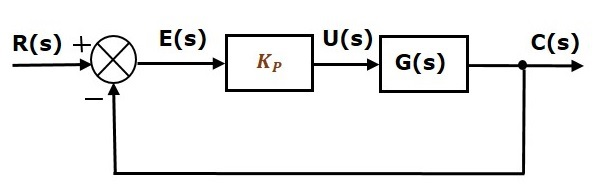
\includegraphics[scale=0.6]{Immagini/Controllori/Pschema}
		\caption{Schema teorico controllore proporzionale}
		\label{fig:Pschema}
	\end{center}
\end{figure}
L'azione proporzionale è utile in quanto più grande è l'errore all'ingresso del controllore e maggiore sarà l'azione svolta da esso. Il regolatore, riprendendo l'equazione \ref{eq:PID} si può notare che solo con il contributo proporzionale la velocità di risposta del sistema aumenta, però con guadagno elevato diminuisce la stabilità e quindi aumentano le oscillazioni\footnote{Il parametro proporzionale viene definito ed analizzato molto in letteratura, nella pratica però è solo un parametro teorico, infatti solitamente si fa riferimento alla banda proporzionale, definita come la variazione minima dell'ingresso che porta l'uscita al valore minimo percentuale.}.
Viene mostrata ora l'implementazione del controllore:
\begin{figure}[ht]
	\begin{center}
		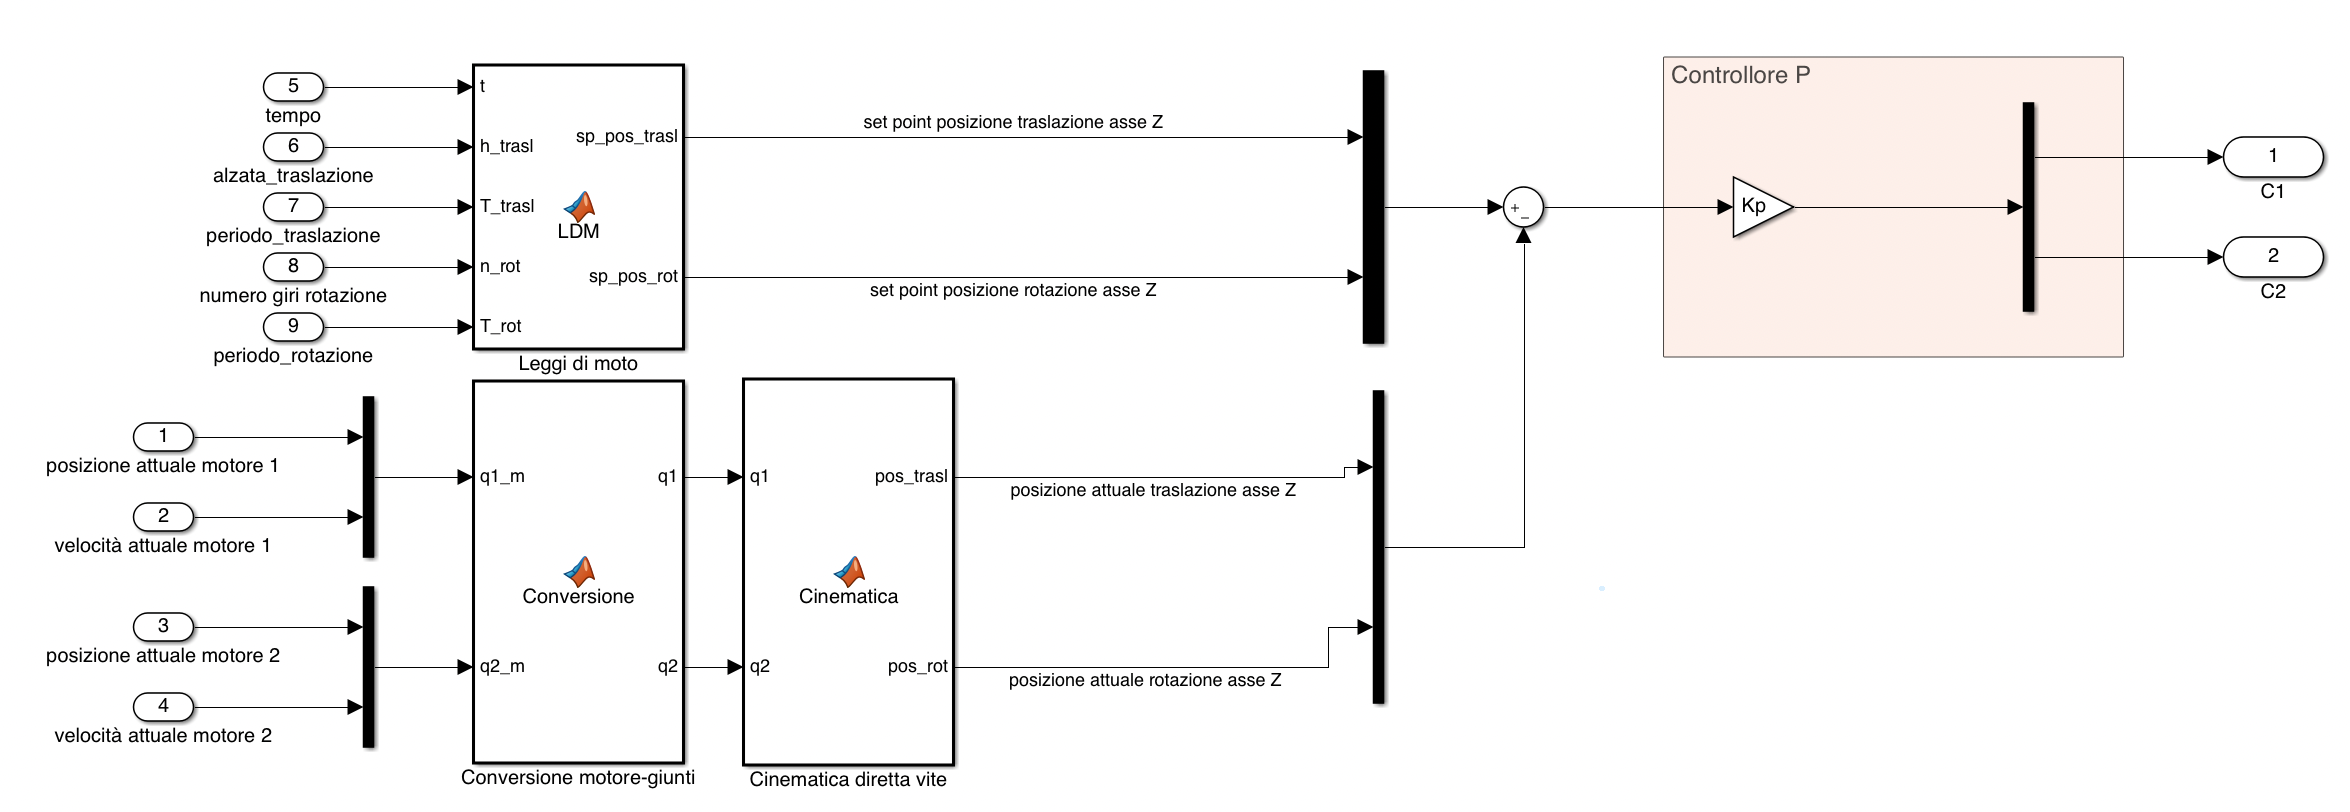
\includegraphics[scale=0.37]{Immagini/Controllori/ViteP}
		\caption{Controllore proporzionale vite}
		\label{fig:PVite}
	\end{center}
\end{figure}
\\Il movimento effettuato è composto da una discesa di 5 centimetri in contemporanea ad una rotazione di $360^\circ$ in due secondi.
\begin{figure}
	\begin{subfigure}{.5\textwidth}
		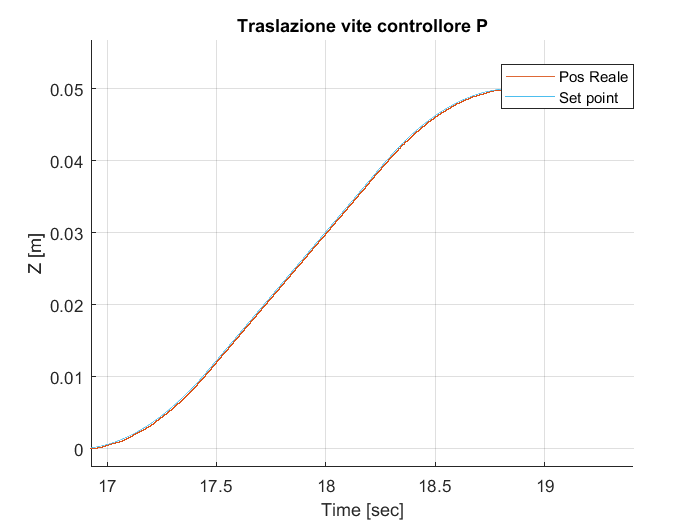
\includegraphics[width=1\linewidth]{Immagini/Traiettorie/TrasViteP}  
		\caption{Traslazione vs riferimento}
		\label{fig:sub-v0}
	\end{subfigure}
	\begin{subfigure}{.5\textwidth}
		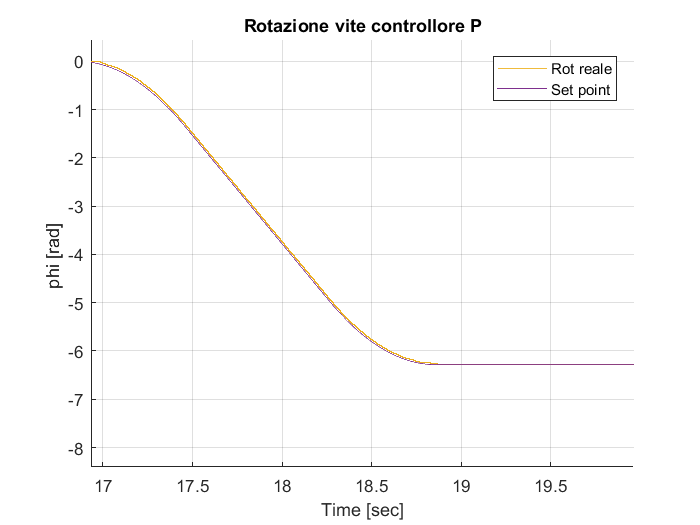
\includegraphics[width=1\linewidth]{Immagini/Traiettorie/RotViteP}  
		\caption{Rotazione vs riferimento}
		\label{fig:sub-v01}
	\end{subfigure}
	\caption{Andamento vite rispetto a riferimento}
	\label{fig:ViteP}
\end{figure}
\subsubsection{Controllo proporzionale derivativo}
A partire dal controllore precedente l'idea è quella di aggiungere una parte: l'azione derivativa. In uscita fornisce la derivata rispetto al tempo dell'errore, se dovessimo analizzarla singolarmente potremmo definire una legge del tipo:
\begin{equation}
\tau_v = K_D\dot{q}_v
\end{equation}
Vi è la presenza della velocità, infatti il controllore derivativo viene anche chiamato controllore di velocità, il suo comportamento è sostanzialmente diverso da quello proporzionale in quanto l'uscita dipende dalla velocità con la quale varia l'errore e riesce a fornire un anticipo di fase. Riprendendo l'equazione \ref{eq:PID} il parametro che controlla questo anticipo è $T_D$ infatti nel caso in cui $K_P=K_I=0$ andando ad analizzare solo il suo comportamento si nota che la stabilità del sistema peggiora sia aumentando che diminuendo il valore. Andando ora ad unire i due contributi si ottiene un controllore PD.
\begin{figure}[ht]
	\begin{center}
		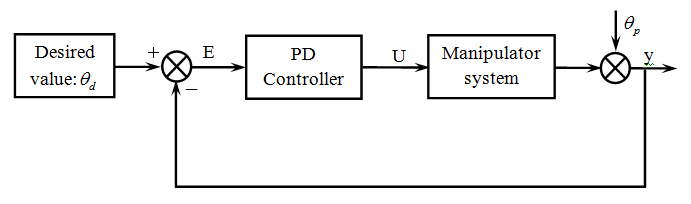
\includegraphics[scale=0.35]{Immagini/Controllori/PDSchema}
		\caption{Schema teorico controllore PD }
		\label{fig:PDSchema}
	\end{center}
\end{figure}
È possibile scrivere l'azione combinata dei due controllori considerando il rapporto ingresso uscita e ottenendo:
\begin{equation}
\tau_v = K_P(1+sT_D)
\end{equation}
con $T_D = \frac{K_D}{K_P}$. In caso di ingresso definito come uno scalino, la presenza del termine derivativo va ad introdurre uno zero e ad aumentare il coefficiente di s, andando a ridurre le oscillazioni e di conseguenza stabilizzando il sistema.\\ A livello implementativo viene presentato lo schema del controllore PD:
\begin{figure}[ht]
	\begin{center}
		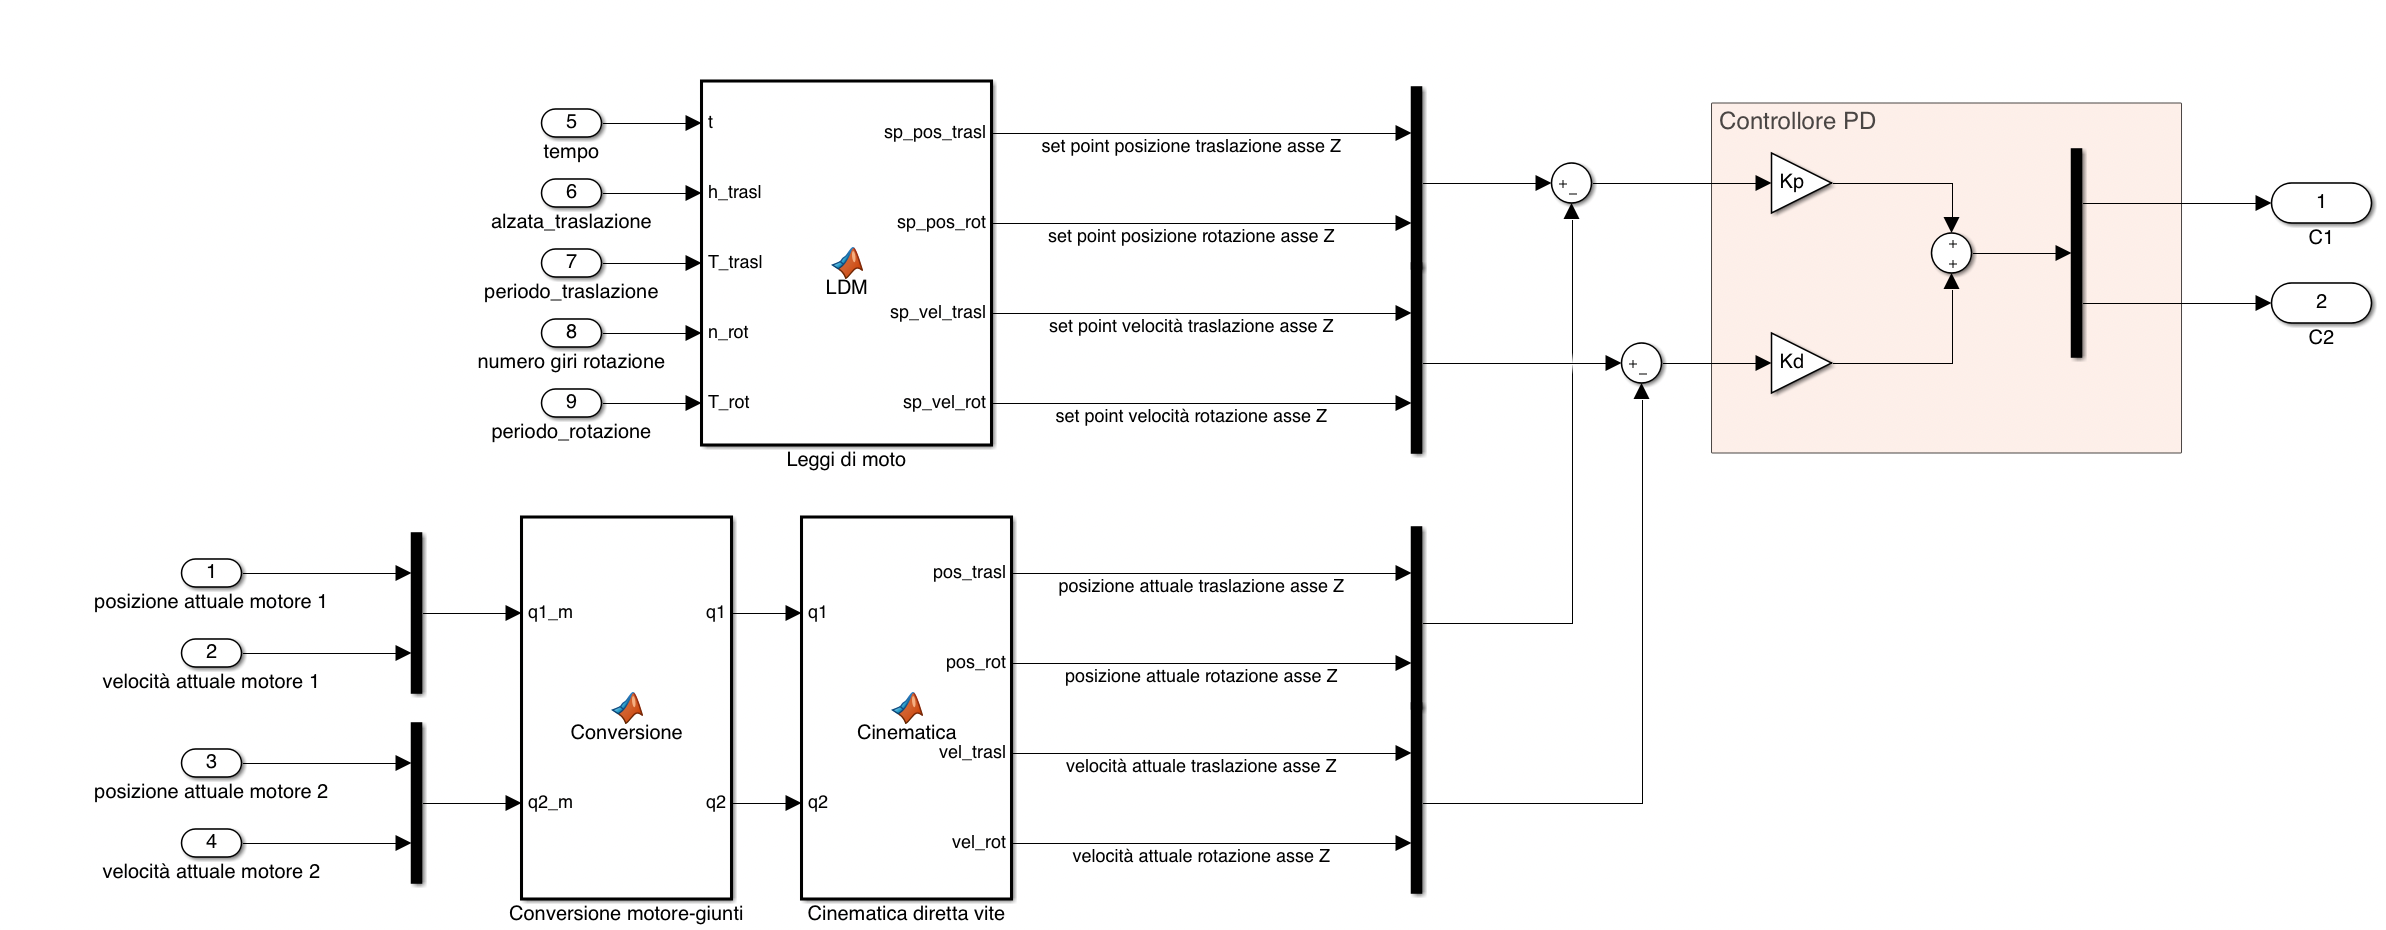
\includegraphics[scale=0.35]{Immagini/Controllori/Vite}
		\caption{Controllore PD Vite}
		\label{fig:PDVite}
	\end{center}
\end{figure}
\\A partire da una legge di moto per entrambi i motori che fornisce quattro set point, si hanno: una prima fase di raccolta dei dati nei quali si prendono le posizioni e velocità dei motori della vite, essendo i motori connessi a riduttori, ed operando sui giunti vi è un blocco che si occupa di fare la conversione;  vi è poi la necessità di effettuare la cinematica diretta per poter passare dagli angoli alle coordinate dell'asse z. In seguito verrà fatta una differenza tra le posizioni e velocità per poter trovare gli errori. Questi, verranno poi moltiplicati per $K_p$ (posizione) e $K_d$ (velocità) per ottenere i valori della legge di controllo da assegnare ai motori.
Viene presentato ora il risultato di una simulazione di una traiettoria che comprendeva la discesa della vite in due secondi di 5 centimetri ed in contemporanea una rotazione di $360^\circ$.
\begin{figure}
	\begin{subfigure}{.5\textwidth}
		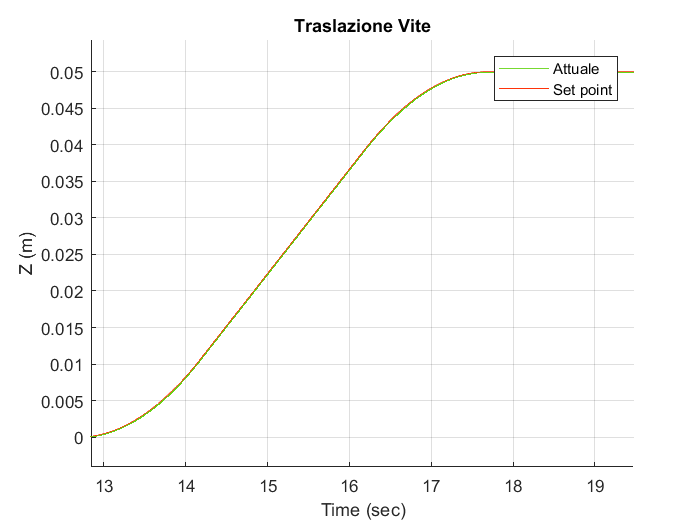
\includegraphics[width=1\linewidth]{Immagini/Traiettorie/TrasVitePD}  
		\caption{Traslazione vs riferimento}
		\label{fig:sub-v1}
	\end{subfigure}
	\begin{subfigure}{.5\textwidth}
		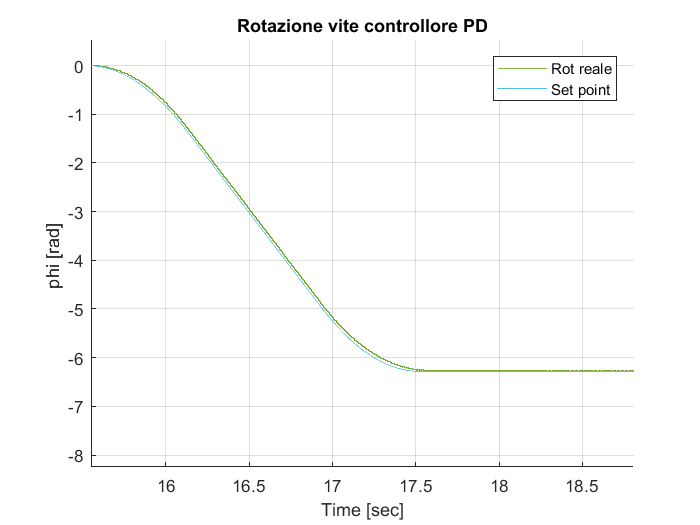
\includegraphics[width=1\linewidth]{Immagini/Traiettorie/RotVitePD}  
		\caption{Rotazione vs riferimento}
		\label{fig:sub-v2}
	\end{subfigure}
	\caption{Andamento vite rispetto a riferimento}
	\label{fig:ViteMovimenti}
\end{figure}
\subsubsection{Confronto controllori vite}	
Nei grafici seguenti è mostrato il confronto fra gli errori di traslazione e rotazione tra i due approcci di controllo implementati per la vite in figura \label{fig:errVite}.
\begin{figure}
	\begin{subfigure}{.5\textwidth}
		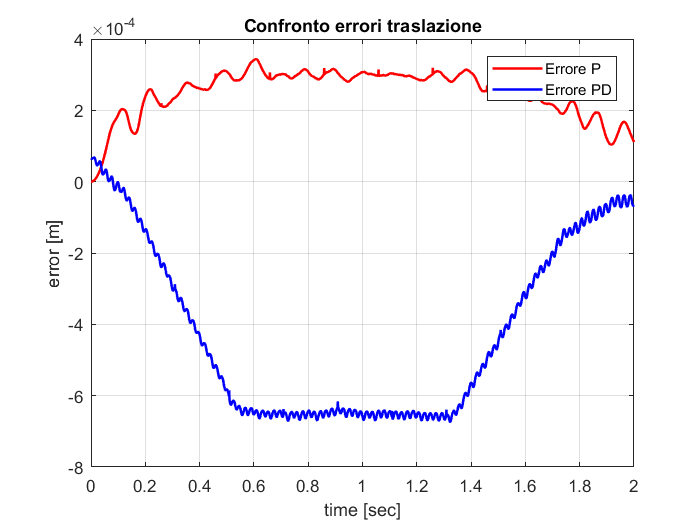
\includegraphics[width=1\linewidth]{Immagini/Traiettorie/errTras}  
		\caption{Errore traslazione}
		\label{fig:sub-errT}
	\end{subfigure}
	\begin{subfigure}{.5\textwidth}
		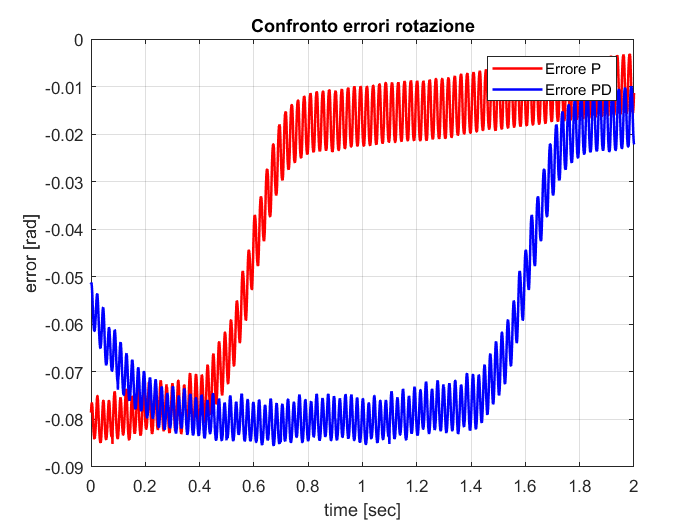
\includegraphics[width=1\linewidth]{Immagini/Traiettorie/errRot}  
		\caption{Errore rotazione}
		\label{fig:sub-errR}
	\end{subfigure}
	\caption{Errori controllori vite}
	\label{fig:errVite0}
\end{figure}
A differenza del controllore P quello PD integra la velocità, seguendo questo approccio le traiettorie hanno un ritardo minore; il problema principale è che la velocità ricevuta in output dagli azionamenti presenta vibrazioni e di conseguenza il controllo risulta imperfetto. Per la scelta del controllore bisogna fare un \textit{trade-off} tra ritardo e vibrazioni.
\subsection{Controllo braccia}
Questa sottosezione si pone come obiettivo l'introduzione di approcci di controllo noti in letteratura e applicarli ai link motorizzati del manipolatore; in particolare andando ad analizzare il loro funzionamento a livello teorico, la loro implementazione pratica ed i risultati ottenuti, cercando quindi il controllore migliore. Tutte le tipologie di controllo introdotte saranno di tipo centralizzato, gli algoritmi di questa tipologia sfruttano una conoscenza più approfondita del modello dinamica del manipolatore in modo tale da compensare i termini di accoppiamento non lineari, verranno quindi introdotte coppie di compensazione per i termini NL, inoltre, qualsiasi incertezza della struttura e qualunque imprecisione nella misura della posizione daranno origine ad una perdita di accuratezza e quindi a problemi di controllo. %A differenza dei controllori della vite, la metodologia utilizzata per la spiegazione teorica in questo caso non includerà le funzioni di trasferimento, verterà però su metodi di Lyapunov e sui concetti di equilibrio.
\subsubsection{Controllo proporzionale derivativo}
La prima tipologia di controllo applicata è stata quella proporzionale derivativa. L'obiettivo di questa tecnica è quello di risolvere il problema della regolazione, ovvero assegnare la posizione corretta all'end-effector rispetto ad un riferimento di equilibrio costante. Non viene risolto il problema della dinamica con la quale si raggiunge quella configurazione, però come l'obiettivo è il trovare la struttura del controllore che assicuri una stabilità asintotica in quella specifica posa desiderata. Viene definito lo stato come: 
\begin{equation}
\tilde{q} = q^0_m - q_m
\end{equation}
Con $q^0_m$ che rappresenta il \textit{set-point} (posizione desiderata) e $q_m$ la posizione attuale, per poter andare a risolvere il problema è necessario di introdurre il metodo diretto di Lyapunov, il quale dice che: 
\begin{center}
\textit{L’analisi della stabilità di un punto di equilibrio viene fatta utilizzando, oltre alle equazioni di stato del sistema, opportune funzioni scalari, dette funzioni di Lyapunov, definite sullo spazio degli stati. }
\end{center}
Si definisce quindi la funzione come:
\begin{equation}
V(\dot{q:m},\tilde{q}) = \frac{1}{2} \dot{q_m}M(q_m)\dot{q_m} + \frac{1}{2} \tilde{q}K_p \tilde{q} >0
\end{equation}
Il termine $K_p$ rappresenta la rigidezza del sistema ed è una matrice $(n x n)$ simmetrica e definita positiva. Considerando che il \textit{set-point} è un termine costante si può andare a derivare la funzione V rispetto al tempo ottenendo:
\begin{equation*}
\dot{V} = \ddot{q_m}M(q_m)\dot{q_m}+\frac{1}{2} \dot{q_m}\dot{M}(q_m)\dot{q_m}-\dot{q_m}K_p\tilde{q}
\end{equation*}
e sapendo che $\tau_m = M(q_m)\ddot{q_m} + C(q_m,\dot{q_m)})\dot{q_m}$\footnote{Nella trattazione di Lyapunov appare anche il termine di compensazione gravitazionale però nel manipolatore analizzato questo termine è costante e pari a zero.} La funzione viene riscritta come: 
\begin{equation}
\dot{V} = \dot{q_m} [\tau_m - K_p \tilde{q}]
\label{eq:finLap}
\end{equation}
Considerando la legge di controllo PD definita come:
\begin{equation}
\tau_m = K_p\tilde{q} - K_d\dot{q_m}
\end{equation}
e andando a sostituirla nell'equazione \ref{eq:finLap} si ottiene:
\begin{equation*}
\dot{V} = -\dot{q_m}K_d \dot{q_m} \le 0
\end{equation*}
Se $K_d$ è una matrice definita positiva allora $\dot{V}$ è semidefinita negativa, la dinamica del sistema è quindi:
\begin{equation}
M(q_m)\ddot{q_m} + C(q_m,\dot{q_m})\dot{q_m} = K_p\tilde{q}-K_d\dot{q_m}
\end{equation}
In particolare le velocità e le accelerazioni sono nulle in corrispondenza di $\dot{V} = 0$. Lo schema teorico di controllo è uguale a quello visto in figura \ref{fig:PDSchema} nella sezione della vite.
\\ Viene mostrato ora lo schema di controllo implementato sul manipolatore:
\begin{figure}[ht]
	\begin{center}
		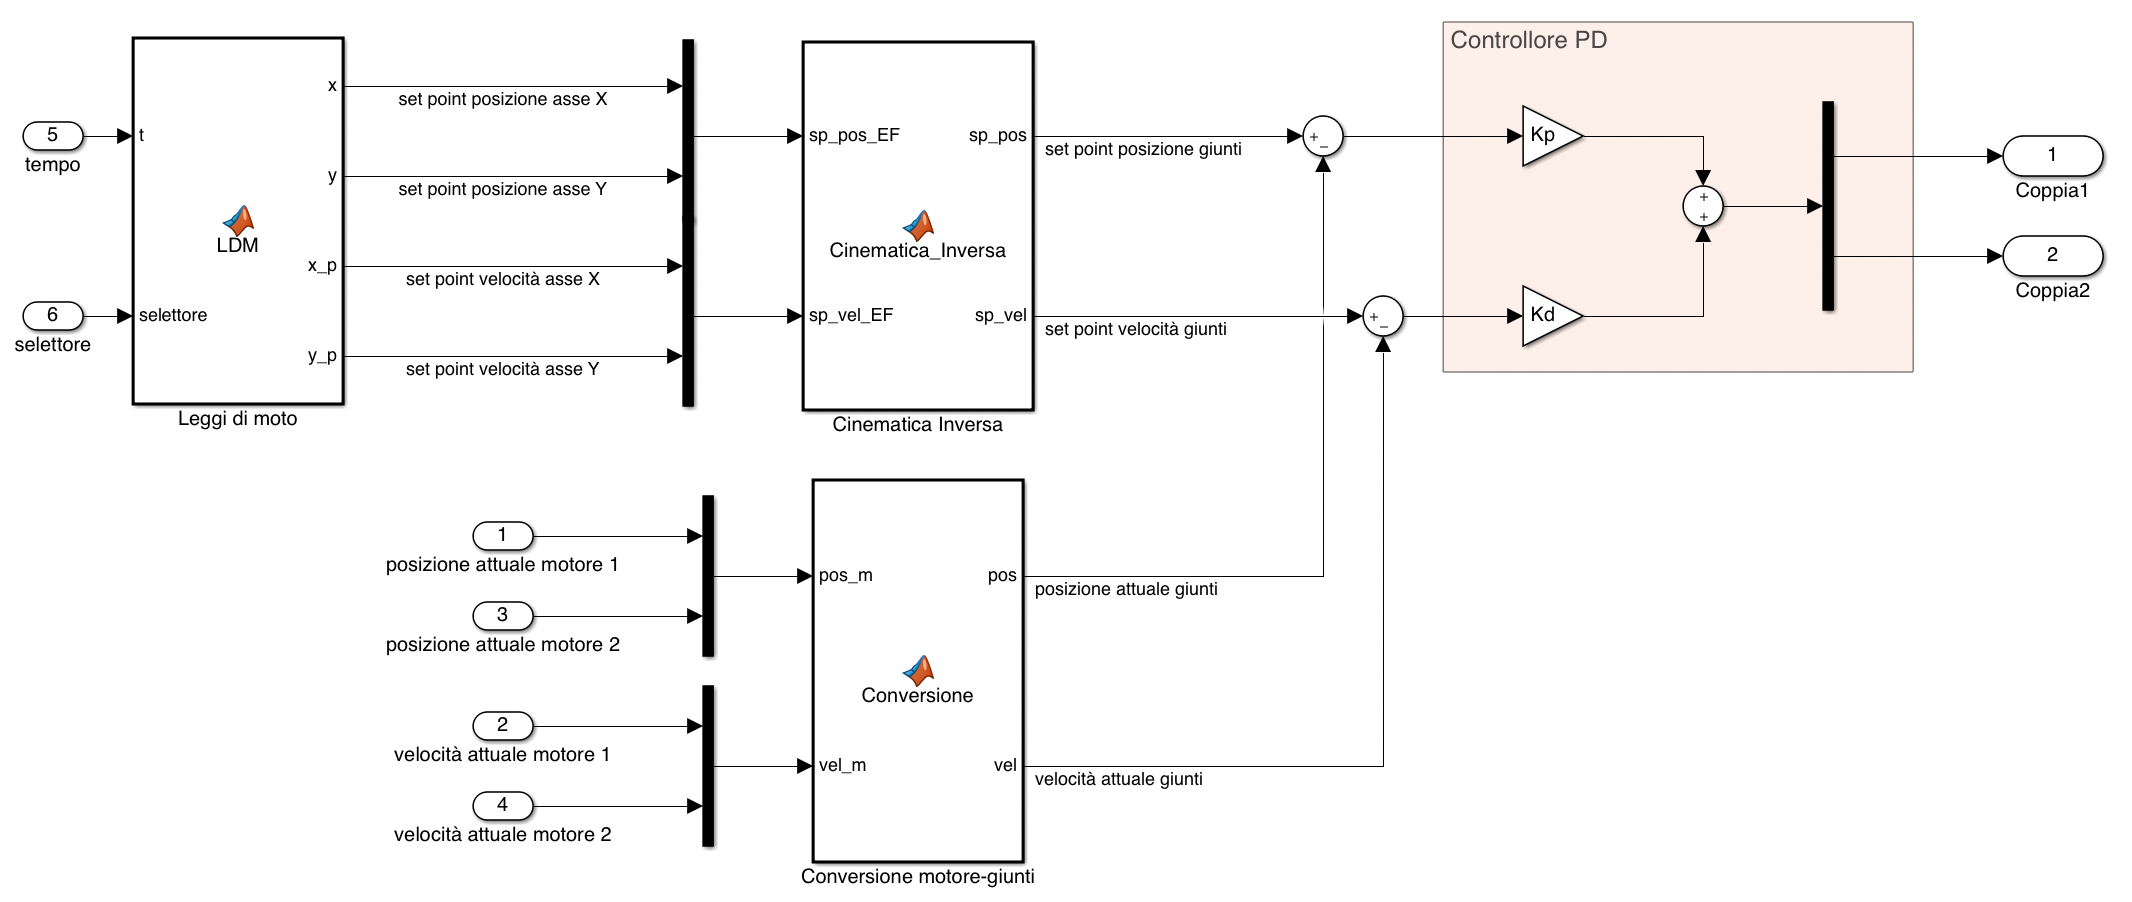
\includegraphics[scale=0.37]{Immagini/Controllori/PDBraccia}
		\caption{Controllore PD braccia}
		\label{fig:PDBraccia}
	\end{center}
\end{figure}
Avendo la possibilità di scegliere tra più traiettorie, a partire dal tempo attuale e dalla traiettoria desiderata si definisce una legge di moto che fornirà i \textit{set-point} in posizione, velocità all'end-effector. Per andare a convertire questi in coordinate ai giunti vi è un blocco che si occupa di fare la cinematica inversa. Vengono poi lette le posizioni e velocità attuali dei motori e verranno successivamente convertite ai giunti; avendo ora tutto a livello di giunti è possibile fare la differenza tra riferimento e reale ottenendo un errore in posizione e uno in velocità\footnote{gli errori sono dei vettori $[2x1]$ contenenti le due componenti relative ai due angoli $\theta_1, \theta_2$.}. Gli errori verranno moltiplicati per $K_p$ e $K_d$ per ottenere la legge di controllo che verrà assegnata ai motori.
\par Per poter andare a testare il controllore è stata assegnata una legge di moto che disegna un cerchio di raggio $5cm$ in 5 secondi. In figura vengono mostrate le coppie assegnate ai giunti $\theta_1$ e $\theta_2$:
\begin{figure}[!ht]
\begin{subfigure}{.5\textwidth}
  \centering
  % include first image
  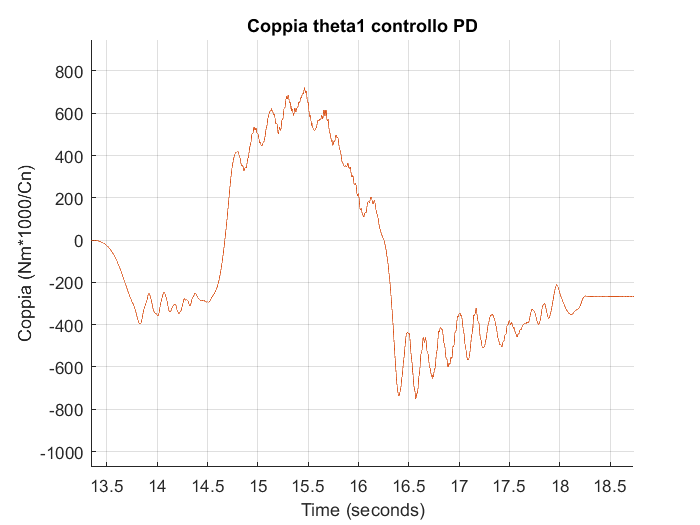
\includegraphics[width=1\linewidth]{Immagini/Traiettorie/CoppiaT1PD}  
  \caption{Coppia $\theta_1$ controllore PD}
  \label{fig:sub-coppiaPD1}
\end{subfigure}
\begin{subfigure}{.5\textwidth}
  \centering
  % include second image
  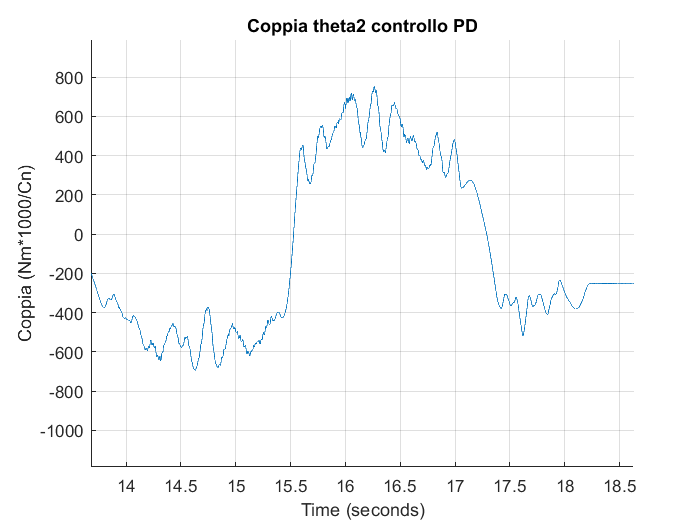
\includegraphics[width=1\linewidth]{Immagini/Traiettorie/CoppiaT2PD}  
  \caption{Coppia $\theta_2$ controllore PD}
  \label{fig:sub-coppiaPD2}
\end{subfigure}
\caption{Coppie controllore PD braccia}
\end{figure}
\\È possibile andare ad analizzare la posizione ottenuta con quelle coppie rispetto al riferimento, e di conseguenza trovare anche l'errore:
\begin{figure}[!ht]
\begin{subfigure}{.5\textwidth}
  \centering
  % include first image
  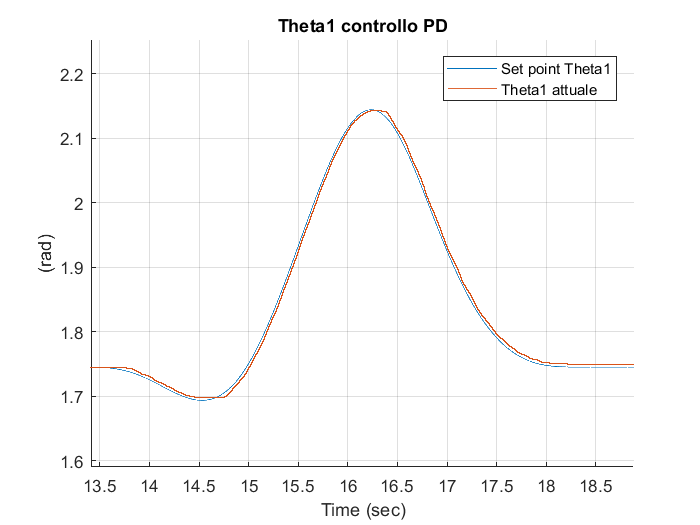
\includegraphics[width=1\linewidth]{Immagini/Traiettorie/Theta1PD}  
  \caption{$\theta_1$ reale vs setpoint}
  \label{fig:sub-pd1p}
\end{subfigure}
\begin{subfigure}{.5\textwidth}
  \centering
  % include second image
  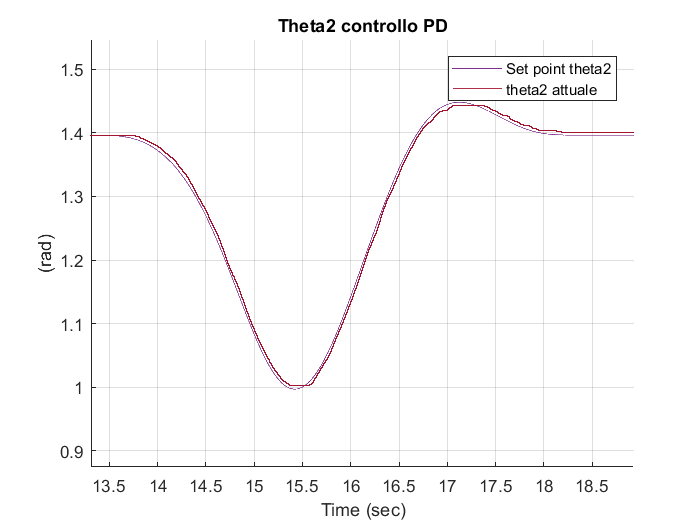
\includegraphics[width=1\linewidth]{Immagini/Traiettorie/Theta2PD}  
  \caption{$\theta_2$ reale vs setpoint}
  \label{fig:sub-pd2p}
\end{subfigure}
\begin{subfigure}{.5\textwidth}
  \centering
  % include third image
  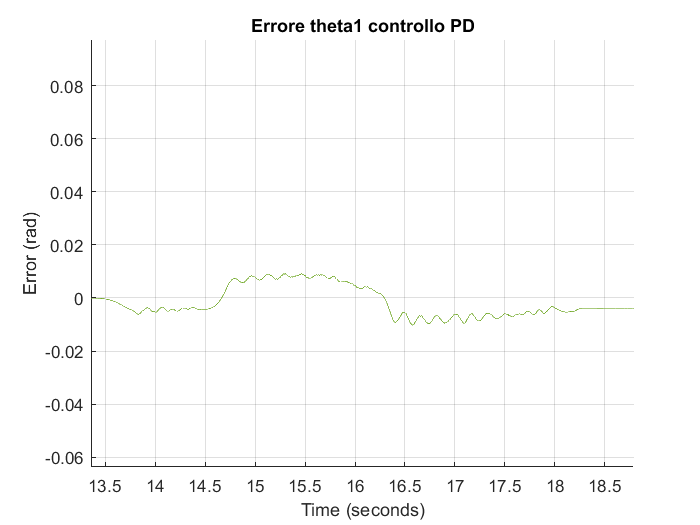
\includegraphics[width=1\linewidth]{Immagini/Traiettorie/ErroreTheta1PD}  
  \caption{Errore su $\theta_1$}
  \label{fig:sub-pd3p}
\end{subfigure}
\begin{subfigure}{.5\textwidth}
  \centering
  % include third image
  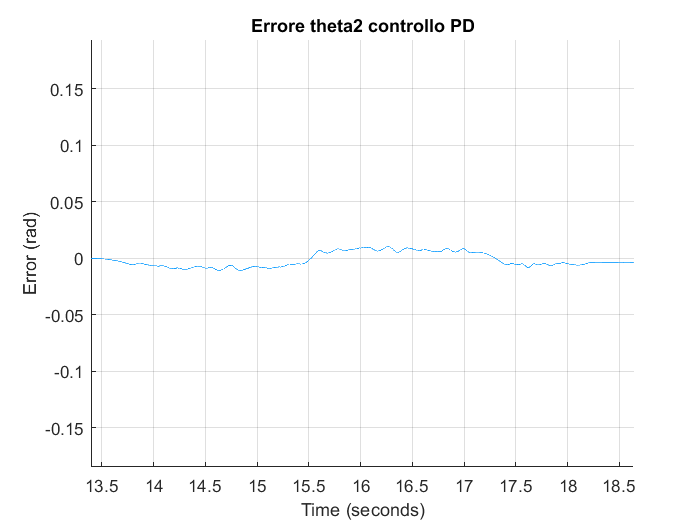
\includegraphics[width=1\linewidth]{Immagini/Traiettorie/ErroreTheta2PD}  
  \caption{Errore su $\theta_2$}
  \label{fig:sub-pd4p}
\end{subfigure}
\caption{Andamenti posizione ed errori controllore PD}
\label{fig:AndamentiPD}
\end{figure}
\\Per una maggior chiarezza vengono rappresentati la traiettoria reale e il riferimento anche sull'asse [X,Y] in figura \ref{fig:PDBracciaC}
\begin{figure}[ht]
	\begin{center}
		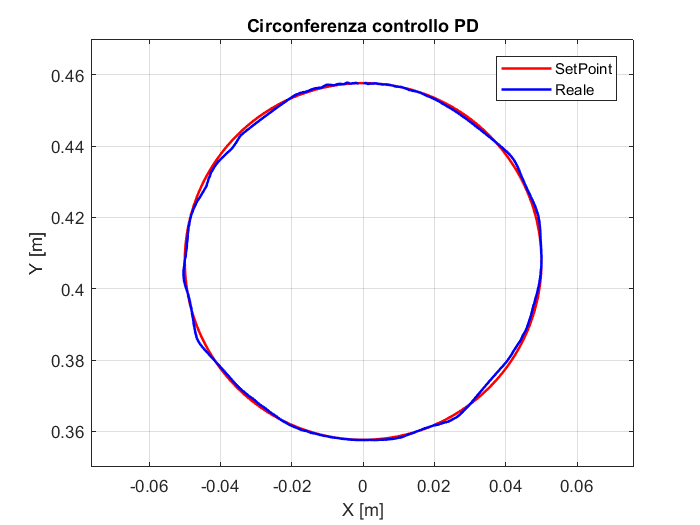
\includegraphics[scale=0.42]{Immagini/Traiettorie/Cerchio}
		\caption{Cerchio assi  [x,y] controllore PD}
		\label{fig:PDBracciaC}
	\end{center}
\end{figure}
\subsubsection{Controllo feed-forward con coppia pre-computata}
Il passo successivo è stato quello di studiare ed implementare un controllore che opera in anello aperto; in particolare questo controllore calcola le coppie di disturbo basate sul modello matematico del sistema con parametri d'ingresso il \textit{set-point} in posizione e velocità e accelerazione. L'introduzione di questi termini riesce a risolvere in maniera corretta il problema del tracciamento della traiettoria desiderata, di conseguenza gli elementi introdotti riescono a compensare gli effetti di accoppiamento presenti nel modello dinamico del sistema. 
\begin{equation}
g_d = \Delta M(q^0_m)\ddot{q_m}^0 + C(q^0_m,\dot{q_m^0})\dot{q_m^0}
\end{equation}
L'idea è che i termini vengono calcolati considerando i valori di posizione, velocità ed accelerazione del rifermento, poiché grazie ad una legge di moto sono sempre ben noti. L'elemento $g_d$ compensa i termini di accoppiamento non lineari dovuti a forza d'inerzia, di Coriolis e centrifughe che dipendono dalla struttura e di conseguenza variano durante il movimento del manipolatore; in generale però calcolare questo termine è molto impegnativo, di conseguenza l'utilizzo di questo approccio su un sistema online può richiedere molto tempo, per questo solitamente vengono compensati solo i termini più importanti come quelli inerziali.
\begin{figure}[ht]
	\begin{center}
		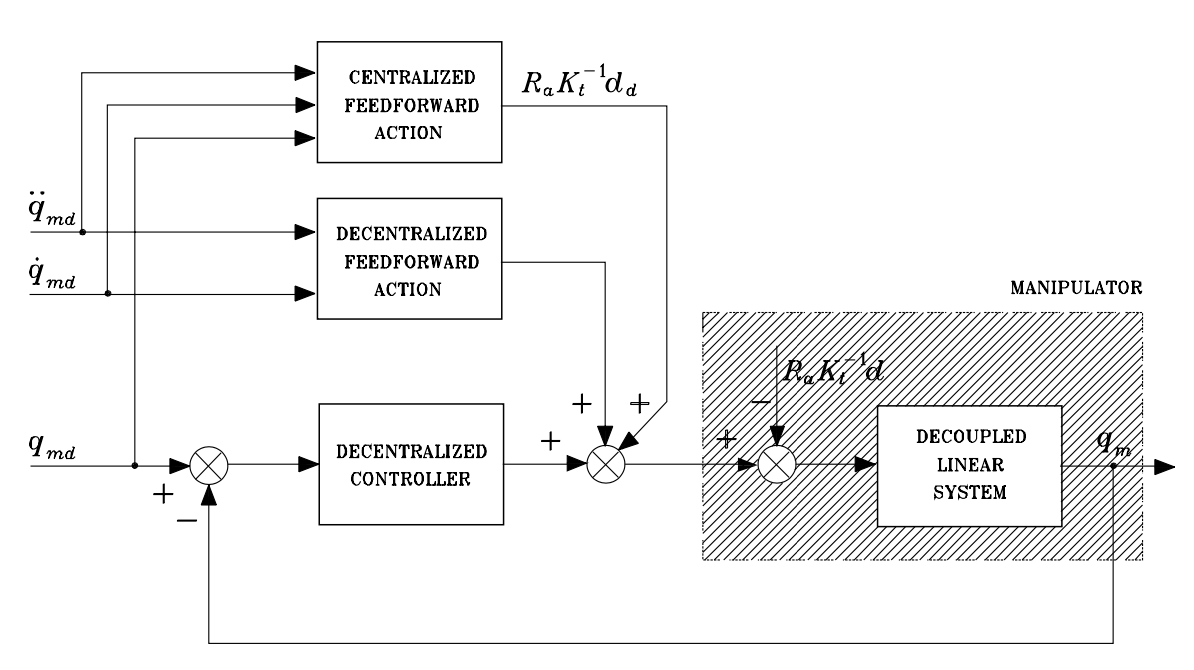
\includegraphics[scale=0.45]{Immagini/Controllori/FFschema}
		\caption{Schema teorico controllo feedforward}
		\label{fig:FFschema}
	\end{center}
\end{figure}
\\A livello implementativo è possibile vederlo come:
\begin{figure}[ht]
	\begin{center}
		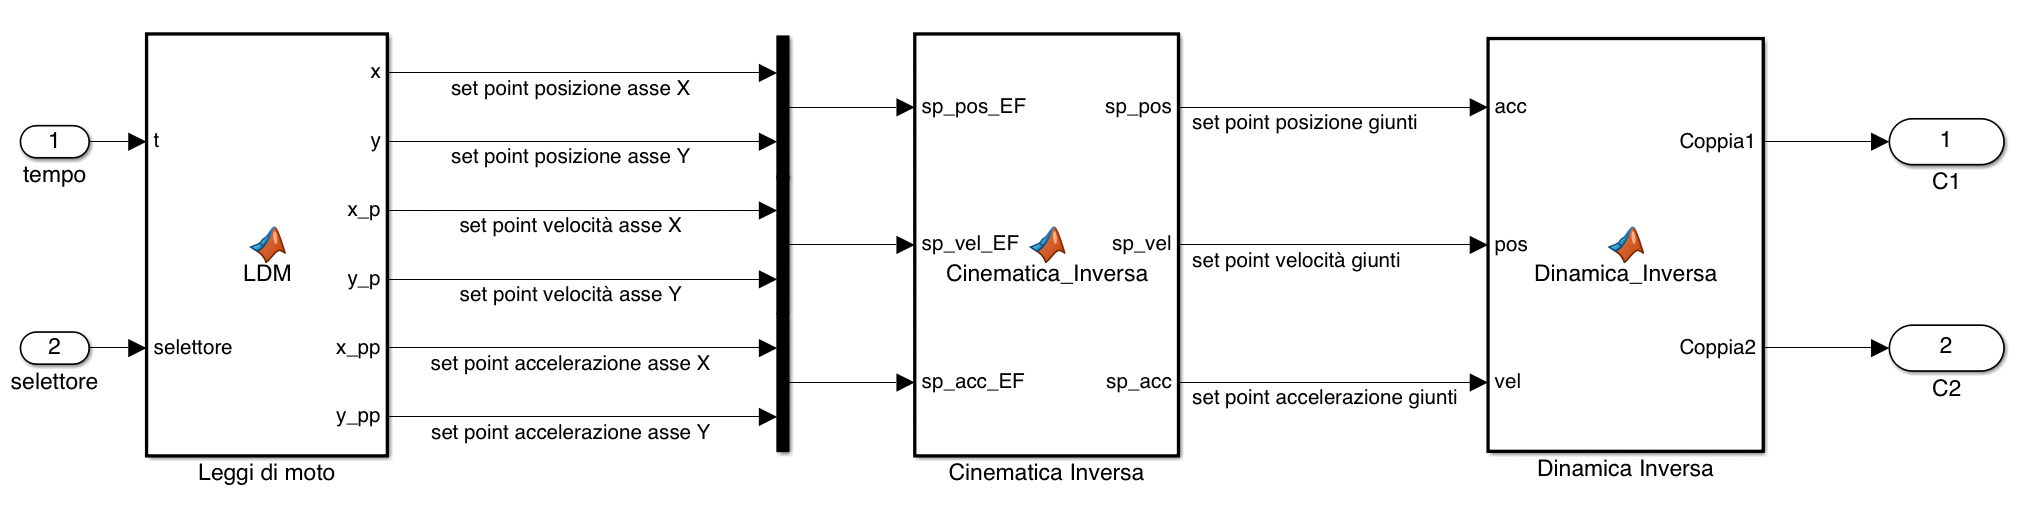
\includegraphics[scale=0.35]{Immagini/Controllori/feedForward}
		\caption{Controllore feedforward}
		\label{fig:FF}
	\end{center}
\end{figure}
\\A partire dalla legge di moto selezionata si ottengono i \textit{set-point} all'end-effector, che grazie alla cinematica inversa vengono convertiti in riferimento ai giunti.  Una volta ottenuti i riferimenti di posizione, velocità ed accelerazione si va ad applicare la funzione di dinamica inversa per calcolare le coppie necessarie. Le coppie sono quindi calcolate esclusivamente mediante dai riferimenti, è possibile vedere questo controllore come una versione di quello a dinamica inversa in anello aperto.
\begin{figure}[ht]
	\begin{center}
		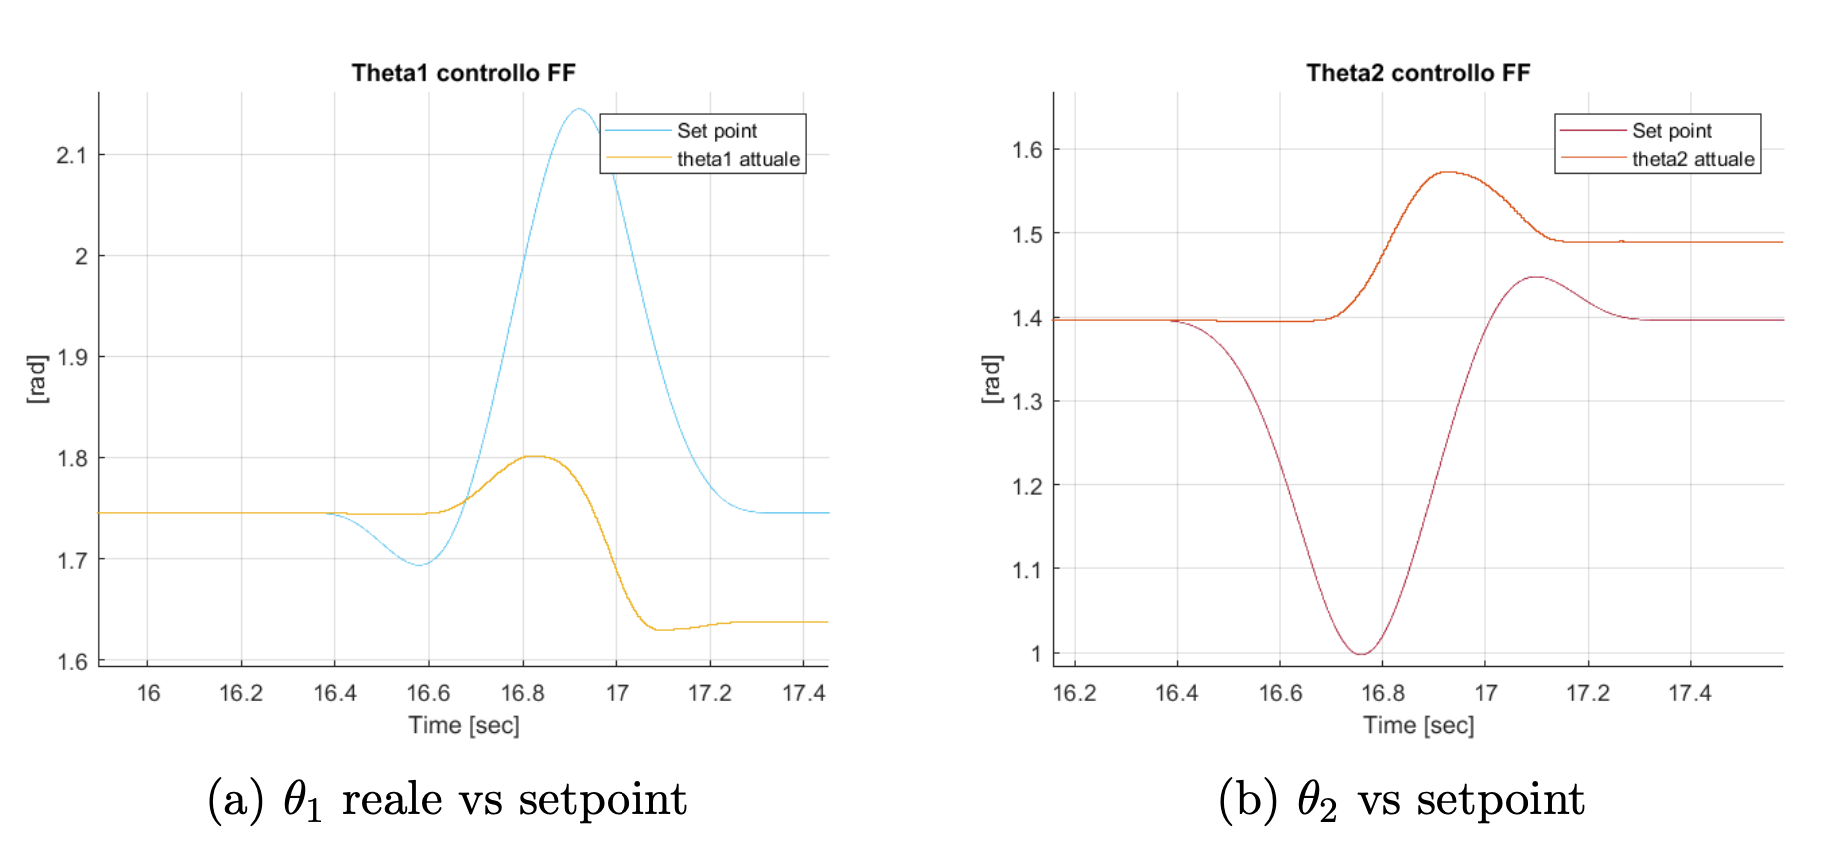
\includegraphics[scale=0.45]{Immagini/Traiettorie/fftot}
\caption{Andamenti controllo feed-forward}
		\label{fig:ffcoppie}
	\end{center}
\end{figure}
Eseguendo traiettorie con una dinamica maggiore, con una conseguente diminuzione del tempo di esecuzione il manipolatore riesce ad eseguire un movimento, però non segue la traiettoria desiderata; questo è dovuto alla mancata stima degli attriti nel modello considerato.
\subsubsection{Controllo in dinamica inversa}
Riprendendo le tecniche di controllo centralizzato caratteristiche della letteratura l'approccio successivo è stato quello del controllo in dinamica inversa. Il primo \textit{step} è stato quello di prendere l'equazione della dinamica e ridefinirla come: 
\begin{equation}
M(q_m)\ddot{q_m} + n(q_m,\dot{q_m}) = \tau_m
\label{eq:ControlloreID}
\end{equation}
Dove $n(q_m,\dot{q_m})$ raccoglie i termini centrifughi e di Coriolis (in letteratura raccoglie anche i termini gravitazionali, ma come anticipato precedentemente nel caso preso in considerazione equivalgono a zero). L'idea del controllo a dinamica inversa si basa sul trovare il vettore di coppie $\tau_m$ come funzione dello stato del sistema, cercando di creare una relazione ingresso-uscita di tipo lineare. Considerando che l'equazione della dinamica è lineare nel controllo e che la matrice d'inerzia è invertibile in ogni configurazione del manipolatore si ha la garanzia di trovare un controllore linearizzato di questo tipo. È possibile andare a riscrivere il controllo come:
\begin{equation}
\tau_m = M(q_m)y + n(q_m,\dot{q_m})
\end{equation}
Dove $y = \ddot{q_m}$ rappresenta un vettore d'ingresso con espressione ancora da determinare. La legge di controllo è basata sul calcolo della dinamica inversa del manipolatore, il sistema è lineare e disaccoppiato rispetto al nuovo ingresso, questo implica che le componenti $y_k$ con $k = -\infty \dots m-1$ influenzano solo la variabile $q_m$ indipendentemente dal movimento degli altri giunti. In questo modo il problema del controllo è quello di trovare una legge \textbf{y} stabilizzante. Viene quindi scelta:
\begin{equation}
y = K_p\tilde{q} + K_d\tilde{\dot{q}}+\ddot{q}_m^0
\label{eq:yID}
\end{equation}
Dove con i termini $\tilde{q}$ e $\tilde{\dot{q}}$ si indica la differenza tra il \textit{setpoint} e la misurazione attuale di posizione e velocità. 
\begin{equation}
\tilde{q} = q^0_m - q_m \ \ \  \tilde{\dot{q}}= \dot{q}^0_m-\dot{q}_m
\label{eq:Tilde}
\end{equation}
Si possono sostituire le definizioni di \ref{eq:Tilde} in \ref{eq:yID} trovando l'espressione:
\begin{equation}
\tilde{\ddot{q}} + K_d + \tilde{\dot{q}} = 0
\end{equation}
Chiaramente l'errore si verifica quando uno o entrambi i termini sono diversi da zero.  Però, volendo assegnare la dinamica a ciascun giunto basta selezionare  i guadagni delle matrici $K_p$ e $K_d$ , inoltre, se le due matrici sono definite positive è possibile ottenere un sistema asintoticamente stabile. 
È possibile scegliere le matrici come:
\begin{equation*}
K_p = diag(\omega^2_{01}, \dots, \omega^2_{0n}) \overline{M} \ \ \  K_d = diag(2 \xi_1 \omega_{01}, \dots ,2 \xi_n \omega_{0n}) \overline{M} 
\end{equation*}
Grazie al controllo a dinamica inversa i termini di compensazioni vengono calcolati ad ogni iterazione, quindi a piccoli intervalli temporali, il loop interno serve per ottenere una relazione ingresso/uscita lineare e disaccoppiata mentre quello esterno grazie alla dinamica desiderata serve a stabilizzare il sistema.
\begin{figure}[ht]
	\begin{center}
		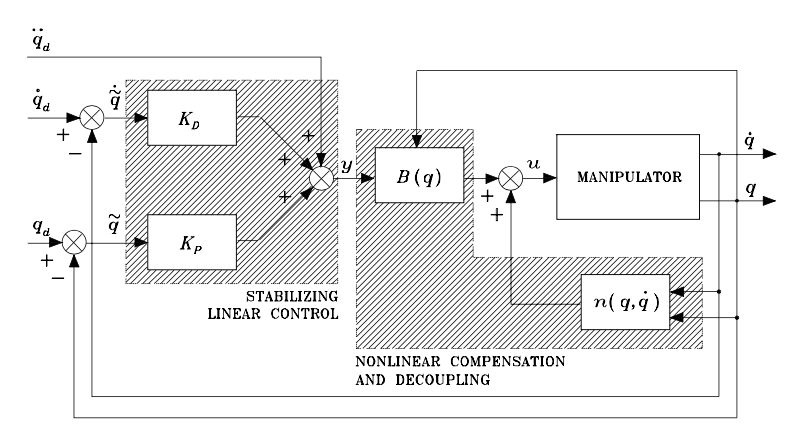
\includegraphics[scale=0.9]{Immagini/Controllori/IDTeoria}
		\caption{Schema controllore dinamica inversa}
		\label{fig:IDBraccia}
	\end{center}
\end{figure}
L'utilizzo di questo approccio è basato sull'ipotesi della cancellazione perfetta dei termini dinamici, quindi, i parametri dinamici del sistema devono essere accuratamente conosciuti e l'equazione del moto deve essere calcolata in real-time. In figura viene presentato lo schema implementato sul controllore come:
\begin{figure}[ht]
	\begin{center}
		\includegraphics[scale=0.32]{Immagini/Controllori/SchemaID}
		\caption{Controllore dinamica inversa}
		\label{fig:IDRBraccia}
	\end{center}
\end{figure}
Come per tutti i controllori visti fino ad ora a partire da selettore e dal tempo ed applicando la cinematica inversa  si ottengono i riferimenti di posizione,  velocità ed accelerazione; andando poi a prendere le posizioni e le velocità attuali dei motori e le convertendole da motori ai giunti. Successivamente per posizione e velocità si vanno a trovare gli errori che verranno moltiplicati rispettivamente per $K_p$ e $K_d$. Per ottenere la y bisogna sommare questi due componenti insieme all'accelerazione del riferimento. Una volta ottenuto questo si va ad applicare la funzione di dinamica inversa con ingressi pari a $ID(y,q,\dot{q})$, da questa è possibile ottenere la legge di controllo e le relative coppie che andranno assegnate ai link del manipolatore. 
\subsubsection*{Test Kp e Kd}
\addcontentsline{toc}{subsubsection}{Test Kp e Kd}
Per andare a scegliere $K_p$ e $K_d$ in modo preciso è stato adottato un approccio sperimentale, ovvero far variare $K_p$, in un range di valori compreso ad incrementi di 50, in base ad un valore fisso di $K_d$. La legge di moto selezionata è stata quella del cerchio in cinque secondi, una legge molto lenta andando ad analizzare quando il controllo iniziava a dar origine a vibrazioni. Si può vedere in figura \ref{fig:KdTest} un risultato di questo metodo, dai test condotti si vede che all'aumentare di entrambi i parametri le vibrazioni iniziano a crescere, e sono visibili prima  
\begin{figure}[!ht]
\begin{subfigure}{.5\textwidth}
  \centering
  % include first image
  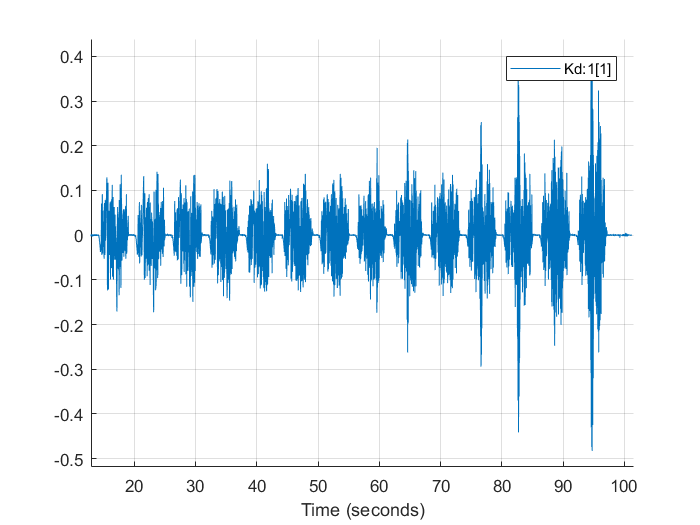
\includegraphics[width=.85\linewidth]{Immagini/Sperimentale/Test_Kd=15.png}  
  \caption{Test con $K_d$ = 1.5}
  \label{fig:sub-kd1.5}
\end{subfigure}
\begin{subfigure}{.5\textwidth}
  \centering
  % include third image
  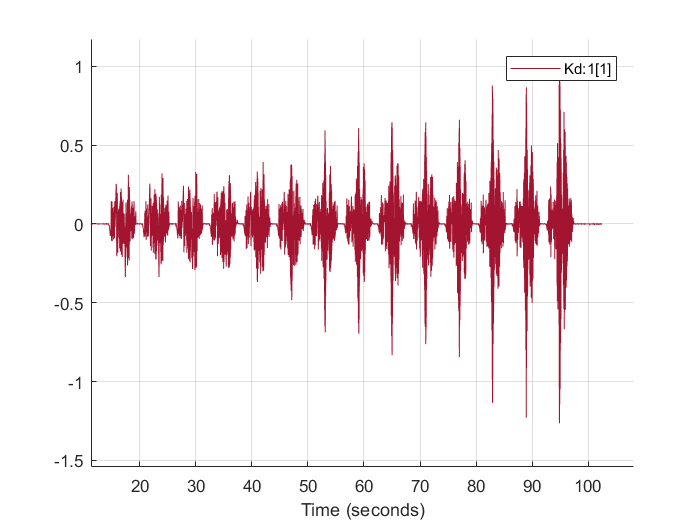
\includegraphics[width=.85\linewidth]{Immagini/Sperimentale/Test_Kd=3.png}  
  \caption{Test con $K_d$=3}
  \label{fig:sub-kd3}
\end{subfigure}
\caption{Ricerca di $K_d$ al variare di $K_p$}
\label{fig:KdTest}
\end{figure}
\subsubsection*{Analisi}
Anche in questo caso, come nei precedenti la traiettoria principale testata è stata quella del cerchio raggio 5cm in 5 secondi, vengono presentate le coppie fornite ai giunti,
\begin{figure}
\begin{subfigure}{.53\textwidth}
  % include third image
  \includegraphics[width=.9\linewidth]{Immagini/Traiettorie/CoppiaT1ID}  
  \caption{Coppia $\theta_1$}
  \label{fig:sub-ikd1}
\end{subfigure}
\begin{subfigure}{.53\textwidth}
  % include third image
  \includegraphics[width=.9\linewidth]{Immagini/Traiettorie/CoppiaT2ID}  
  \caption{Coppia $\theta_2$}
  \label{fig:sub-ikd2}
\end{subfigure}
\caption{Coppie giunti controllo dinamica inversa}
\label{fig:CoppieID}
\end{figure}
come per il controllore PD è possibile andare a vedere e comparare la posizione attuale rispetto al riferimento e trovare l'errore:
\begin{figure}[!ht]
\begin{subfigure}{.53\textwidth}
  \centering
  % include first image
  \includegraphics[width=.9\linewidth]{Immagini/Traiettorie/Theta1ID}  
  \caption{$\theta_1$ reale vs \textit{setpoint}}
  \label{fig:sub-id1}
\end{subfigure}
\begin{subfigure}{.53\textwidth}
  \centering
  % include second image
  \includegraphics[width=.9\linewidth]{Immagini/Traiettorie/Theta2ID}  
  \caption{$\theta_2$ reale vs setpoint}
  \label{fig:sub-pd2k}
\end{subfigure}
\caption{Posizione vs riferimento controllore ID}
\end{figure}
\begin{figure}
\begin{subfigure}{.53\textwidth}
  \centering
  % include third image
  \includegraphics[width=.9\linewidth]{Immagini/Traiettorie/ErroreTheta1ID}  
  \caption{Errore su $\theta_1$}
  \label{fig:sub-pd3k}
\end{subfigure}
\begin{subfigure}{.5\textwidth}
  \centering
  % include third image
  \includegraphics[width=.9\linewidth]{Immagini/Traiettorie/ErroreTheta2ID}  
  \caption{Errore su $\theta_2$}
  \label{fig:sub-pd4}
\end{subfigure}
\caption{Errori controllore ID}
\label{fig:AndamentiID}
\end{figure}
\\Come per il controllore PD anche qua è possibile andare a rappresentare la traiettoria nel piano cartesiano, ottenendo:
\begin{figure}[ht]
	\begin{center}
		\includegraphics[scale=0.6]{Immagini/Traiettorie/CerchioDinamicaInversa}
		\caption{Cerchio [X,Y] controllo ID}
		\label{fig:IDbracciaC}
	\end{center}
\end{figure}
\subsubsection{Controllo robusto}
 L'effetto di incertezze sul modello induce in errore il sistema di controllo, soprattutto nel caso reale bisogna supporre che la compensazione del modello dinamico risulti imperfetta magari a causa di approssimazioni oppure per semplificazioni.  L'equazione \ref{eq:ControlloreID} può essere riscritta come:
\begin{equation}
\tau_m = \hat{M}(q_m)y + \hat{n}(q_m,\dot{q}_m)
\end{equation}
Dove $\hat{M}$ e $\hat{n}$ rappresentano i parametri stimati del modello dinamico, è possibile rappresentare l'incertezza come:
\begin{equation*}
\overline{M} = \hat{M}- M \ \ \overline{n} = \hat{n} - n
\end{equation*}  
Riprendendo la legge di controllo vista precedentemente, viene riscritta come:
\begin{equation}
M(q_m)\ddot{q}_m + n(q_m,\dot{q_m}) = \hat{M}(q_m)y + \hat{n}(q_m,\dot{q_m})
\end{equation}
Essendo la matrice M invertibile in ogni configurazione è possibile ricavare $\ddot{q}_m$:
\begin{equation*}
\ddot{q}_m = y + (M^{-1}\hat{M}-I)y+M^{-1}\tilde{n} = y-\eta
\end{equation*}
Dove $\eta$ è una funzione non lineare definita come: \begin{equation}
\eta = (I-M^{-1}\hat{M})y - M^{-1}\tilde{n} 
\end{equation}
Adottando la legge \ref{eq:Tilde} vista nel caso del controllore a dinamica inversa si ottiene che l'errore dinamico è gestito dall'equazione:
\begin{equation}
\ddot{\tilde{q}} + K_d \dot{\tilde{q}} + K_p\tilde{q} = \eta
\end{equation}
Il risultato è quindi un sistema non lineare e accoppiato, di conseguenza implementare un semplice controllore PD non basta; per risolvere questo problema occorre inserire un termine non lineare, che sia funzione dell'errore e creato appositamente per fornire robustezza al controllo. Come per il controllore PD si ricerca una funzione grazie al metodo diretto di Lyapunov. 
\\Viene definito lo stato del sistema come:
\begin{equation*}
\xi = \begin{bmatrix}
\tilde{q} \\ \dot{\tilde{q}}
\end{bmatrix}
\end{equation*}
sostituendo poi lo stato nell'equazione $\ddot{q}_m = y-\eta$ si ottiene un'equazione differenziale del primo ordine
\begin{equation}
\dot{\xi} = H\xi + D(\ddot{q}_m^0 - y + \eta)
\end{equation}
Dove H e D sono definite come:$H = \begin{bmatrix}
0 & I \\ 0 & 0
\end{bmatrix} \in \mathbb{R}^{(2nx2n)}$ , $D = \begin{bmatrix}
0 \\ I
\end{bmatrix} \in \mathbb{R}^{(2nxn)}$
\\Si può vedere il problema di inseguimento della traiettoria come la soluzione che va a stabilizzare il sistema non lineare di qui sopra. Nella letteratura del controllore robusto, anche se l'incertezza $\eta$ non è nota è comunque disponibile un suo intervallo di variazione. La legge \textbf{y} dovrebbe garantire stabilità di $\dot{\xi}$ per ogni $\eta$ nell'intervallo. Di conseguenza vengono formulate tre assunzioni:
\begin{enumerate}
\item $\sup_{t\ge 0} ||\ddot{q}^0_m || < Q_M < \infty \forall \ddot{q}_m^0$
\item $||I-M^{-1}\hat{M}(q_m)|| \le \alpha \le 1 \forall q_m$
\item $||\tilde{n}|| \le \Phi(||\xi||) < \infty \forall q_m, \dot{q}_m$
\end{enumerate}
Andando ad analizzare le assunzioni si può dire che:
\begin{itemize}
\item La prima assunzione è soddisfatta sempre, in quanto per ogni traiettoria definita le accelerazioni non possono essere infinite
\item La seconda assunzione conferma che M  (e di conseguenza $M^{-1}$) sia superiormente e inferiormente limitata, infatti 
\begin{equation}
0 < M_m < ||M^{-1}(q_m)|| \le M_M < \infty \forall q_m
\end{equation}
\end{itemize}
Quindi, esiste sempre una scelta di $\hat{M}$ che soddisfa la condizione, selezionando per esempio
\begin{equation*}
\hat{M} = \frac{2}{M_M+M_m}I
\end{equation*} 
ottenendo
\begin{equation}
||M^{-1}(q_m)\hat{M}(q_m)-I|\le \alpha = \frac{M_M-M_m}{M_M+M_m} <1
\end{equation}
Il limite inferiore si ha quando $\hat{M} = M$ in quanto $\alpha = 0$. Andando a concentrarsi sull'assunzione 3, si può osservare che $\tilde{n}$ è funzione di $q_m,\dot{q_m}$, nel primo caso, in base alla tipologia di giunto (rotoidale o prismatico) si hanno intervalli che sono limitati e quindi il contributo è limitato. Anche la velocità è limitata grazie all'effetto della saturazione (esistente sulle velocità massime dei motori). Di conseguenza, prendendo per $\Phi$ una funzione calcolata nella norma dello stato come:
\begin{equation}
\Phi(||\xi||) = \alpha_0 + \alpha_1 ||\xi|| + \alpha_2 ||\xi||^2
\end{equation}
Andando a riprendere la legge di controllo\ref{eq:yID} ed ampliandola è possibile ridefinirla come: 
\begin{equation}
y = \ddot{q}^0_m + K_p\tilde{q} + K_d\dot{\tilde{q}} + \omega
\label{eq:yRob}
\end{equation}
Il termine PD assicura la stabilizzazione della dinamica della matrice dell'errore, $\ddot{q}^0_m$ fornisce un termine di previsione e $\omega$ è progettato in modo da combattere l'incertezza fornendo robustezza al sistema.
\begin{equation}
\dot{\xi} = \tilde{H}\xi + D(\eta-\omega)
\end{equation}
Dove:
\begin{equation*}
\tilde{H} = H-DK = \begin{bmatrix}
0 & I \\ -K_p & -K_d
\end{bmatrix} \in 
\mathbb{R}^{(2nx2n)}
\end{equation*}
\begin{equation*}
 \ K_p = diag(\omega^2_{01}, \dots, \omega^2_{0n})  \ \ \  K_d = diag(2 \xi_1 \omega^2_{01}, \dots ,2 \xi_n \omega^2_{0n}) 
\end{equation*}
Per andare a definire $omega$ si procede col metodo diretto di Lyapunov; considerando come funzione:
\begin{equation}
V(\xi) = \xi^TQ\xi >0 , \forall \xi \neq 0
\end{equation}
con Q matrice simmetrica definita positiva. Facendo la derivata lungo la traiettoria si trova che
\begin{equation}
\dot{V} = \xi^T P\xi + 2z^T(\eta-\omega)
\label{eq:LyapDerivRob}
\end{equation}
Considerando che $\tilde{H}$ ha tutti gli autovalori con parte reale negativa, è possibile scegliere una qualunque P definita positiva che soddisfi:
\begin{equation*}
\tilde{H}^TQ+Q\tilde{H} = -P
\end{equation*}
Considerando ora l'equazione \ref{eq:LyapDerivRob} , $z = D^TQ\xi$, il primo termine sulla parte di destra è definito negativo, di conseguenza la soluzione converge solo se $\xi \in \mathbb{N}(D^TQ)$, se invece non appartiene, il controllo $\omega$ andrà scelto per rendere il secondo termine minore o uguale a zero utilizzando la legge di controllo:
\begin{equation}
\omega = \rho(||\xi||)\frac{z}{||z||}, \rho >0
\end{equation}
con $\rho$ funzione positiva da determinare. Scegliendo $\omega$ in questo modo si ottiene:
\begin{equation*}
z^T(\eta-\omega) = z^T\eta - \rho(||\xi||)\frac{zz^T}{||z||} \le ||z||\big[||\eta||.\rho(||\xi||)\big]
\end{equation*}
se poi si garantisce che: $||\xi||>||\eta||$ per ogni valore di posizione, velocità e velocità di riferimento, si ottiene che questo termine e $\dot{V}$ sono negativi lungo tutte le traiettorie dell'errore; per poter soddisfare la disuguaglianza, dalla definizione di $\eta$ è possibile trovare:
\begin{equation}
\eta = (I-M^{-1}\hat{M})y-M^{-1}\tilde{n} \ e \ y = \ddot{q}^0_m + K\xi+\omega
\end{equation}
sapendo poi che $||\omega|| = \rho$ si trova che:
\begin{equation*}
||\eta|| \le ||I-M^{-1}\hat{M}|| (||\ddot{q}_m^0 ||+||K||\  ||\xi||+||\omega||)+||M^{-1}|| \ ||\tilde{n}||
\end{equation*}
Andando a maggiorare questa quantità si ottiene:
\begin{equation}
||\eta|| \le \alpha Q_M + \alpha ||K|| || \xi || + \alpha\rho(||\xi||)+M_M\Phi(||\xi||) < \rho(||\xi||)
\end{equation}
è quindi possibile andare a selezionare un $rho$ in modo tale che:
\begin{equation}
\rho(||\xi||) \ge \frac{1}{1-\alpha} [\alpha Q_M+\alpha ||K|| ||\xi||+M_M\Phi(||\xi||)]
\label{eq:HelpRho}
\end{equation}
Si può osservare che $\Phi(||\xi||) = \alpha_0+\alpha_1||\xi||+\alpha_2||\xi||^2$ per soddisfare \ref{eq:HelpRho} basta che si selezionino:
\begin{equation*}
\rho(||\xi||) = \beta_0 + \beta_1||\xi||+\beta_2||\xi||^2
\end{equation*}
Con i valori:
\begin{equation*}
\begin{cases}
\beta_0 \ge \frac{\alpha Q_M+\alpha_0M_M}{1-\alpha}\\
 \beta_1 \ge \frac{\alpha K +\alpha_1 M_M}{1-\alpha}\\
 \beta_2 \ge \frac{\alpha_2M_M}{1-\alpha}
\end{cases}
\end{equation*}
Andando poi a sostituire tutto nell'equazione \ref{eq:LyapDerivRob} si trova:
\begin{equation}
\dot{V} = -\xi^T P \xi + 2z^T(\eta-\rho(||\xi||) \frac{z}{||z||}) <0 \ \forall
\xi \neq 0
\end{equation}
Di conseguenza $\xi = 0$ è un equilibrio di stato asintoticamente e globalmente stabile. La legge di controllo è quindi formata da tre termini, un primo termine che compensa i termini non lineari e gli accoppiamenti tra i link, un secondo termine che stabilizza il sistema dinamico grazie ad una retroazione con previsione per l'errore e un terzo termine che fornisce robustezza contrastando le incertezze e calcolando i termini non lineari che dipendono dallo stato del manipolatore. 
\\[15pt]
\par Ad alte frequenze però potrebbe esserci la commutazione della variabile di controllo, che potrebbe portare ad un'elevata presenza di "sali/scendi" a causa del terzo termine, per questo viene approssimato come:
\begin{equation}
\omega = \begin{cases}
\rho(||\xi||) \frac{z}{||z||} \ for\ ||z||\ge \varepsilon \\
\rho(||\xi||) \frac{z}{\varepsilon} \ \ \ for \ ||z|| < \varepsilon
\end{cases}
\label{eq:epsilon}
\end{equation}
Viene rappresentato ora lo schema del controllo robusto teorico come:
\begin{figure}[ht]
	\begin{center}
		\includegraphics[scale=0.8]{Immagini/Controllori/RobustTeoria}
		\caption{Schema controllore robusto}
		\label{fig:RobustSchema}
	\end{center}
\end{figure}
Data la difficoltà implementativa del controllore robusto sul modello reale è state condotta un'analisi e simulazione del controllore sul modello simulink del manipolatore.
\subsubsection*{Implementazione controllore robusto}
\addcontentsline{toc}{subsubsection}{Implementazione controllore robusto}
L'implementazione su simulink del controllore robusto consiste nel seguente schema: 
\begin{figure}[ht]
	\begin{center}
		\includegraphics[scale=0.5]{Immagini/Controllori/RobustSchema}
		\caption{Controllore robusto}
		\label{fig:robustSchema}
	\end{center}
\end{figure}
Anche per questo approccio è stata condotta un'analisi su una traiettoria circolare di raggio 5 cm da eseguire in 3 secondi. Di rilevanza in tutti questi test è stato il parametro $\varepsilon$, visto nell'equazione \ref{eq:epsilon} si presentano ora i risultati all'uscita del controllo robusto, andando a concentrarsi sui parametri zV e le coppie di controllo ottenute al variare del parametro $\varepsilon$.
Si può vedere che per valori di $\varepsilon$ relativamente piccoli il valore di zV presenta alti fenomeni vibratori causati dalla commutazione ad alta frequenza della variabile di controllo.
\begin{figure}[!ht]
	\begin{subfigure}{.53\textwidth}
		\centering
		% include first image
		\includegraphics[width=.8\linewidth]{Immagini/Traiettorie/epsilon25uscita}  
		\caption{zV con $\varepsilon = 2.5\cdot 10^{-4}$ }
		\label{fig:rob1}
	\end{subfigure}
	\begin{subfigure}{.53\textwidth}
		\centering
		% include second image
		\includegraphics[width=.8\linewidth]{Immagini/Traiettorie/epsilon5uscita}  
		\caption{zV con $\varepsilon = 5\cdot 10^{-5}$}
		\label{fig:rob2}
	\end{subfigure}
	\caption{Uscite parte robusta del controllo}
\end{figure}
\\Per quanto riguarda le coppie di controllo, si può facilmente notare che nel primo caso non vibrano in quanto la variabile d'uscita dal controllo robusto non presenta vibrazioni, nel secondo caso invece le coppie in uscita sono vibrate e questo non le rende ideali per il controllo.
\begin{figure}[!ht]
	\begin{subfigure}{.53\textwidth}
		\centering
		% include first image
		\includegraphics[width=.8\linewidth]{Immagini/Traiettorie/CoppieRobustoe25}  
		\caption{Coppie di controllo con $\varepsilon = 2.5\cdot 10^{-4}$ }
		\label{fig:rob3}
	\end{subfigure}
	\begin{subfigure}{.53\textwidth}
		\centering
		% include second image
		\includegraphics[width=.8\linewidth]{Immagini/Traiettorie/CoppieRobustoe5}  
		\caption{Coppie di controllo con $\varepsilon = 5\cdot 10^{-5}$}
		\label{fig:rob4}
	\end{subfigure}
	\caption{Coppie in uscita al variare di $\varepsilon$}
\end{figure}
\\A differenza dei controlli precedenti, l'unità di misura della coppia è il $[Nm]$ in quanto questi test sono stati condotti esclusivamente su simulink.
\subsection{Confronto approcci controllori}
Avendo introdotto e verificato le principali tipologie di controllo centralizzato viene fatto ora un confronto andando a vedere quale tra gli approcci analizzati è il migliore. In particolare, sulla traiettoria effettuata viene confrontato l'andamento degli errori tra il controllore proporzionale derivativo e quello a dinamica inversa:
\begin{figure}[!ht]
\begin{subfigure}{.53\textwidth}
  \centering
  % include first image
  \includegraphics[width=.9\linewidth]{Immagini/Traiettorie/ConfontoErroriTheta1}  
  \caption{Confronto errore $\theta_1$ }
  \label{fig:sub-tid1}
\end{subfigure}
\begin{subfigure}{.53\textwidth}
  \centering
  % include second image
  \includegraphics[width=.9\linewidth]{Immagini/Traiettorie/ConfontoErroriTheta2}  
  \caption{Confronto errore $\theta_2$}
  \label{fig:sub-tid2}
\end{subfigure}
\caption{Confronto controllore PD e ID}
\end{figure}
\\Gli errori sono espressi in radianti, il picco di errore è circa due decimi di grado. Da entrambe le immagini è chiaro come il controllore a dinamica inversa risulti migliore. Di conseguenza si è scelto questo come controllore definitivo e sono stati analizzati altri andamenti con leggi di moto diverse al fine di valutarne il comportamento.
\begin{figure}[ht]
	\begin{center}
		\includegraphics[scale=0.46]{Immagini/Traiettorie/QuadratoDinamicaInversa}
		\caption{Quadrato controllo dinamica inversa}
		\label{fig:quadID}
	\end{center}
\end{figure}
\\La prima traiettoria eseguita è stata quella del quadrato, nei lati orizzontali \textit{setpoint} e curva reale sono pressoché uguali, in quelli verticali invece il manipolatore segue ma non alla perfezione, questo è dovuto alla contrapposizione dei motori in fase di lavoro. 
\begin{figure}[ht]
	\begin{center}
		\includegraphics[scale=0.45]{Immagini/Traiettorie/PatternDinamicaInversa}
		\caption{Pattern controllo dinamica inversa}
		\label{fig:patternID}
	\end{center}
\end{figure}
\\La seconda figura è ancora una traiettoria in 2D ed è un pattern di quadrati nei quali il manipolatore non passa mai più di una volta per lo stesso punto, anche qua si può notare, come si è visto in precedenza per il quadrato che i lati orizzontali sono eseguiti correttamente mentre in quelli verticali possono originarsi vibrazioni. Nella parte inferiore si riescono vedere più vibrazioni in quanto come visto [metti ref. a workspace] il numero di condizionamento è più alto e quindi ci si sta avvicinando ad una configurazione singolare.
\begin{figure}[ht]
	\begin{center}
		\includegraphics[scale=0.5]{Immagini/Traiettorie/SpiraleID}
		\caption{Spirale controllo dinamica inversa}
		\label{fig:SpiraleID}
	\end{center}
\end{figure}
\\Come ultima traiettoria si è scelto di eseguirne una tridimensionale: la spirale, in questa è compresa la movimentazione sia delle braccia che della vite, è possibile selezionare quanti cerchi fare e di quanto far scendere la vite; si può vedere che il \textit{setpoint} e la traiettoria reale sono molto simili.
\subsection{Problema della velocità}
Implementando e studiando le tecniche di controllo centralizzato, si può vedere chiaramente come in tutte queste vi è la necessità della velocità $\dot{q}$. Andando a concentrarsi su di essa, notando che la velocità ricavata dagli encoder soffriva di rumore, questa situazione poteva essere critica in quanto un parametro "rumoroso" da origine ad una legge di moto vibrante e di conseguenza non è possibile alzare il contributo $K_d$ in maniera adeguata in quanto aumenterebbero le vibrazioni. Proprio per questo si è scelto di ricercare un metodo che potesse filtrare la velocità o predirla in modo da avere un risultato migliore da poter dare in ingresso al manipolatore.
\subsubsection*{Filtro primo ordine}
\addcontentsline{toc}{subsubsection}{Filtro primo ordine}
L'idea iniziale è stata quella di implementare un filtro del primo ordine passa basso, con funzione di trasferimento:
\begin{equation}
T(s) = \frac{a_0}{s+\frac{b_0}{b_1}} = G_0 \frac{P_0}{s+P_0}
\end{equation}
In questa tipologia di filtri c'è un polo che deve essere reale e negativo per garantire la stabilità (è possibile vedere questa condizione nell'appendice \ref{Appendice:stabilita}). Andando ad analizzare in frequenza l'andamento del filtro $s=j\omega$ si trova che a basse frequenze l'input viene fatto passare completamente, mentre ad alte frequenze viene tagliato.
\begin{figure}[ht]
	\begin{center}
		\includegraphics[scale=0.5]{Immagini/Traiettorie/FiltroIOrdine}
		\caption{Filtro primo ordine}
		\label{fig:filtroIOrd}
	\end{center}
\end{figure}
In figura viene mostrata la velocità reale e due filtri. Il filtro con coefficiente $10^{-2}$ riesce ad approssimare meglio la curva ma è chiaramente in ritardo, invece, il filtro con coefficiente $10^{-3}$ è molto simile alla curva e non riesce a rimuovere le vibrazioni che essa porta.
\subsubsection*{Filtro secondo ordine}
\addcontentsline{toc}{subsubsection}{Filtro secondo ordine}
Un filtro del secondo ordine si differenzia dal primo aggiungendo un polo, permette quindi di arrivare ad avere una pendenza del diagramma di Bode del modulo fino a 40$\frac{dB}{dec}$ nella banda attenuata, mentre in banda passante a seconda dell'approssimazione applicata possono verificarsi vari casi. Dal punto di vista pratico si realizzano mettendo più filtri del primo ordine in serie tra di loro. 
\begin{figure}[ht]
	\begin{center}
		\includegraphics[scale=0.5]{Immagini/Traiettorie/FiltroIIOrdine}
		\caption{Filtro secondo ordine}
		\label{fig:filtroIIOrd}
	\end{center}
\end{figure}
\\In figura si può vedere la velocità reale e tre filtri, anche in questo caso nessuno dei filtri riesce a fornire un output della velocità adeguato. 
\subsubsection*{Filtro di Kalman}
\addcontentsline{toc}{subsubsection}{Filtro di Kalman}
Il filtro di Kalman è un efficiente filtro ricorsivo che valuta lo stato di un sistema dinamico a partire da una serie di misure soggette a rumore, gli approcci implementativi del filtro sono stati due, il primo metodo consisteva nell'approccio al problema mediante tecniche di \textit{sensor fusion}, andando a ricercare i valori delle matrici di covarianza in modo sperimentale e valutando il comportamento del filtro rispetto alla velocità originale; il secondo approccio è stato l'utilizzo del filtro di kalman esteso implementandolo in maniera più teorica.
\subsubsection*{Approccio sensor fusion}
Per l'approccio \textit{sensor fusion} è stato implementato un codice che permette di andare a trovare i valori migliori delle matrici di covarianza. Vengono prima definite le matrici che serviranno per la trattazione e poi riportare ora i due algoritmi fondamentali:
\begin{equation}
A = \begin{bmatrix}
1 & T \\ 0 & 1
\end{bmatrix}, B = \begin{bmatrix}
0 \\ T
\end{bmatrix}, C=\begin{bmatrix}
 1 & 0
\end{bmatrix}, P_0 = \begin{bmatrix}
1 & 0 \\ 0 & 1
\end{bmatrix}
\end{equation}
con $T = 0.001 sec$.  Le variabili incognite che andremo a ricavare sono:
\begin{equation}
R , Q = \begin{bmatrix}
Q_1 & 0 \\ 0 & Q_2
\end{bmatrix}
\end{equation}
\begin{algorithm}
\caption{Creazione del filtro}\label{alg:cap}
\begin{algorithmic}
\For $f \gets 1 : 1000$ \Comment{Costruzione filtro con 1000 punti}
\State $S \gets C\cdot P_m \cdot C^T + R$
\State $K \gets P_m \cdot C'\cdot S^{-1}$
\State $P_p \gets P_m - K\cdot C\cdot P_m$
\State $P_m = A\cdot P_p\cdot A^T + Q$\Comment{Passo di predizione}
\EndFor
\end{algorithmic}
\end{algorithm}
\\Una volta definito il filtro il passo successivo è quello di avviarlo, per far questo vengono fatti \textit{ciclare} i valori di $Q_1,Q_2$ ed R in modo da andare a trovare i migliori: 
\begin{algorithm}
\caption{Avvio filtro}\label{alg:avvio}
\begin{algorithmic}
\Require $Q_1, Q_2, R,Y,\dot{Y}_{rif}$
\For{$i \gets 1 : N$}
\For{$j \gets 1: N$}
\State $Q \gets [Q_1(i),0,0,Q_2(j)]$
\For{$k \gets 1:N$}
\State $r \gets R(k)$
\State $P_m = P_0$
\State $em \gets [0,0]^T$
\For $ g \gets 1 : length(Y)$
\State $ ep \gets em + K\cdot (Y(k)-C*em)$
\State $ [pos,vel] \gets [sep(1),sep(2)]$
 \State $em \gets A\cdot ep + B\cdot Y(k)$
 \State $err(k) \gets \dot{Y}_{rif} - vel$
\EndFor
\For $k \gets 1:length(err)$
\If $mean(abs(err(k)) < my$
\State $my = mean(abs(err(k))$
\State $ Save [i,j,k]$
\EndIf
\EndFor
\EndFor
\EndFor
\EndFor
\end{algorithmic}
\end{algorithm}
Alla fine del ciclo si ottengono i valori di [i,j,k] che permettono di trovare le matrici Q ed R a minimo errore tra riferimento e stima. Grazie alla formula:
\begin{equation}
\frac{|\dot{y}_{rif}-\dot{\hat{y}}|}{N}
\end{equation} 
Per completezza sono stati condotti anche dei test scegliendo come risultato migliore la varianza minore:
\begin{equation}
\sum_{i=0}^{N} \frac{[(\dot{y}_{rif}-\dot{\hat{y}}) - \mu_y]^2}{N}
\end{equation}
Si è visto però che il risultato finale è identico.
\begin{figure}[ht]
	\begin{center}
		\includegraphics[scale=0.52]{Immagini/Kalman1}
		\caption{Kalman \textit{sensor fusion}}
		\label{fig:kalman}
	\end{center}
\end{figure}
\subsubsection*{Filtro di Kalman esteso}
Il filtro di Kalman esteso Extended Kalman Filter (EKF) è una versione non-lineare del filtro di Kalman usata quando l'evoluzione o l'osservazione dello stato del sistema sono non-lineari, un sistema a tempo discreto, non lineare può essere descritto come:
\begin{equation}
	\begin{cases}
		\xi_{k+1} = f(\xi_k,u_k)\\
		y_k = h(\xi_k)
	\end{cases}
\end{equation}
\\Per definire il filtro di Kalman si parte dalla definizione dello stato come
\begin{equation}
\xi = \begin{bmatrix}
\dot{\theta} \\ \theta
\end{bmatrix}
\end{equation}
Si definisce la derivata dello stato come:
\begin{equation}
\dot{\xi} = \begin{bmatrix}
\ddot{\theta} \\ \dot{\theta}
\end{bmatrix} =\begin{bmatrix}
0 & I \\ 0 & -M^{-1}C
\end{bmatrix} + \begin{bmatrix}
0 \\ M^{-1}
\end{bmatrix}\tau_m
\end{equation}
È possibile esprimere questa equazione come:
\begin{equation*}
\dot{\xi} = \varphi(\xi,u)
\end{equation*}
Con u ingresso corrispondente alle coppie. Il filtro, a partire dal valore attuale consente di predire il valore successivo come:
\begin{equation}
\xi_{k+1} - \xi_{k} = \varphi(\xi_k,u_k)\Delta t \rightarrow \xi_{k+1} = \xi_k + \varphi(\xi_k,u_k)\Delta t = f(\xi_k,u_k)
\end{equation}
L'uscita $y_k$ sarà data da: 
\begin{equation}
y_k = \mathbb{F}\xi_k
\end{equation}
Dove:
\begin{equation*}
\mathbb{F} = \frac{\partial f}{\partial \xi} \Bigg|_{\hat{\xi_k},u_k} = \begin{bmatrix}
\frac{\partial f}{\partial \xi_1} & \frac{\partial f}{\partial \xi_2} & \frac{\partial f}{\partial \xi_3} & \frac{\partial f}{\partial \xi_4}
\end{bmatrix}
\end{equation*}
Sfruttando il metodo delle differenze finite(\ref{appendix:diff} è possibile trovare:
\begin{equation}
\frac{\partial}{\partial \xi_d} f(\xi,u) \approx \frac{f(\xi+\Delta\xi\delta_d)-f(\xi-\Delta\xi\delta_d)}{2\Delta\xi}
\end{equation}
Con $\delta_d$ definito come la colonna della matrice identità calcolata col metodo di Sarrus.
\begin{figure}[ht]
	\begin{center}
		\includegraphics[scale=0.52]{Immagini/Kalman2}
		\caption{Filtro di Kalman esteso}
		\label{fig:kalmanek}
	\end{center}
\end{figure}